
%%%%%%%%%%%%%%%%%%%%%%%%%%%%%%%%%%%%%%%%%%%%%%%%%%%%%%%%%%%%%%%%%%%%%%
%%  disstemplate.tex, to be compiled with latex.		     %
%%  08 April 2002	Version 4				     %
%%%%%%%%%%%%%%%%%%%%%%%%%%%%%%%%%%%%%%%%%%%%%%%%%%%%%%%%%%%%%%%%%%%%%%
%%								     %
%%  Writing a Doctoral Dissertation with LaTeX at		     %
%%	the University of Texas at Austin			     %
%%								     %
%%  (Modify this ``template'' for your own dissertation.)	     %
%%								     %
%%%%%%%%%%%%%%%%%%%%%%%%%%%%%%%%%%%%%%%%%%%%%%%%%%%%%%%%%%%%%%%%%%%%%%


\documentclass[12pt]{report}	% The documentclass must be ``report''.

\usepackage{utdiss2}  		% Dissertation package style file.


%%%%%%%%%%%%%%%%%%%%%%%%%%%%%%%%%%%%%%%%%%%%%%%%%%%%%%%%%%%%%%%%%%%%%%
% Optional packages used for this sample dissertation. If you don't  %
% need a capability in your dissertation, feel free to comment out   %
% the package usage command.					     %
%%%%%%%%%%%%%%%%%%%%%%%%%%%%%%%%%%%%%%%%%%%%%%%%%%%%%%%%%%%%%%%%%%%%%%

\usepackage{amsmath,amsthm,amsfonts,amscd} 
				% Some packages to write mathematics.
\usepackage{eucal} 	 	% Euler fonts
\usepackage{verbatim}      	% Allows quoting source with commands.
\usepackage{makeidx}       	% Package to make an index.
\usepackage{graphicx}         	% Allows inclusion of eps files.
\usepackage{epsfig}         	% Allows inclusion of eps files.
%\usepackage{citesort}         	% 
\usepackage{url}		% Allows good typesetting of web URLs.
%\usepackage{draftcopy}		% Uncomment this line to have the
				% word, "DRAFT," as a background
				% "watermark" on all of the pages of
				% of your draft versions. When ready
				% to generate your final copy, re-comment
				% it out with a percent sign to remove
				% the word draft before you re-run
				% Makediss for the last time.


%%%%%%%%%%%%%%%%%%%%%%
%   my own packages
%%%%%%%%%%%%%%%%%%%%%%

\usepackage{wrapfig}
\usepackage{amsmath}
\usepackage{bbold}
\usepackage{subcaption}
\usepackage{xcolor}
\usepackage{natbib}
\usepackage{wrapfig}
\usepackage{float}
\usepackage[ruled, vlined, linesnumbered]{algorithm2e}
\usepackage{scalerel}
\usepackage{dsfont}
\usepackage{hyperref}
\hypersetup{
    colorlinks,
    citecolor=black,
    filecolor=black,
    linkcolor=black,
    urlcolor=black
}
\usepackage{cancel}


\newtheorem{myth}{Theorem}[chapter]
\newtheorem{mylem}{Lemma}[chapter]
\newtheorem{mypro}{Proposition}[chapter]
\newtheorem{mydef}{Definition}[chapter]
\newtheorem{myrem}{Model}
\newtheorem{exem}{Example}[section]


\author{Guy W. Cole}  	% Required

\address{9905 Chukar Circle\\ Austin, Texas 78758}  % Required

% \title{Fairness in Machine Learning and Network-Topic Modeling}
\title{Relational Learning and Fairness}
                                                    % Required

%%%%%%%%%%%%%%%%%%%%%%%%%%%%%%%%%%%%%%%%%%%%%%%%%%%%%%%%%%%%%%%%%%%%%%
% NOTICE: The total number of supervisors and other members %%%%%%%%%%
%%%%%%%%%%%%%%% MUST be seven (7) or less! If you put in more, %%%%%%%
%%%%%%%%%%%%%%% they are put on the page after the Committee %%%%%%%%%
%%%%%%%%%%%%%%% Certification of Approved Version page. %%%%%%%%%%%%%%
%%%%%%%%%%%%%%%%%%%%%%%%%%%%%%%%%%%%%%%%%%%%%%%%%%%%%%%%%%%%%%%%%%%%%%

%%%%%%%%%%%%%%%%%%%%%%%%%%%%%%%%%%%%%%%%%%%%%%%%%%%%%%%%%%%%%%%%%%%%%%
%
% Enter names of the supervisor and co-supervisor(s), if any,
% of your dissertation committee. Put one name per line with
% the name in square brackets. The name on the last line, however,
% must be in curly braces.
%
% If you have only one supervisor, the entry below will read:
%
%	\supervisor
%		{Supervisor's Name}
%
% NOTE: Maximum three supervisors. Minimum one supervisor.
% NOTE: The Office of Graduate Studies will accept only two supervisors!
% 
%
\supervisor
	{Sinead Williamson}

%%%%%%%%%%%%%%%%%%%%%%%%%%%%%%%%%%%%%%%%%%%%%%%%%%%%%%%%%%%%%%%%%%%%%%
%
% Enter names of the other (non-supervisor) members(s) of your
% dissertation committee. Put one name per line with the name
% in square brackets. The name on the last line, however, must
% be in curly braces.
%
% NOTE: Maximum six other members. Minimum zero other members.
% NOTE: The Office of Graduate Studies may restrict you to a total
%	of six committee members.
%
%
\committeemembers
	[Carlos Carvalho]
	[Mingyuan Zhou]
	[Peter Muller]
	{Scott Moser}
	
%%%%%%%%%%%%%%%%%%%%%%%%%%%%%%%%%%%%%%%%%%%%%%%%%%%%%%%%%%%%%%%%%%%%%%

\previousdegrees{ B.S., M.P.P, M.S.}
     % The abbreviated form of your previous degree(s).
     % E.g., \previousdegrees{B.S., MBA}.
     %
     % The default value is `B.S., M.S.'

\graduationmonth{December}      
     % Graduation month, either May, August, or December, in the form
     % as `\graduationmonth{May}'. Do not abbreviate.
     %
     % The default value (either May, August, or December) is guessed
     % according to the time of running LaTeX.

\graduationyear{2019}   
     % Graduation year, in the form as `\graduationyear{2001}'.
     % Use a 4 digit (not a 2 digit) number.
     %
     % The default value is guessed according to the time of 
     % running LaTeX.

%\typist{...}       
     % The name(s) of typist(s), put `the author' if you do it yourself.
     % E.g., `\typist{Maryann Hersey and the author}'.
     %
     % The default value is `the author'.


%%%%%%%%%%%%%%%%%%%%%%%%%%%%%%%%%%%%%%%%%%%%%%%%%%%%%%%%%%%%%%%%%%%%%%
% Commands for master's theses and reports.			     %
%%%%%%%%%%%%%%%%%%%%%%%%%%%%%%%%%%%%%%%%%%%%%%%%%%%%%%%%%%%%%%%%%%%%%%
%
% If the degree you're seeking is NOT Doctor of Philosophy, uncomment
% (remove the % in front of) the following two command lines (the ones
% that have the \ as their second character).
%
%\degree{MASTER OF ARTS}
%\degreeabbr{M.A.}

% Uncomment the line below that corresponds to the type of master's
% document you are writing.
%
%\masterreport
%\masterthesis


%%%%%%%%%%%%%%%%%%%%%%%%%%%%%%%%%%%%%%%%%%%%%%%%%%%%%%%%%%%%%%%%%%%%%%
% Some optional commands to change the document's defaults.	     %
%%%%%%%%%%%%%%%%%%%%%%%%%%%%%%%%%%%%%%%%%%%%%%%%%%%%%%%%%%%%%%%%%%%%%%
%
\singlespacing
%\oneandonehalfspacing

%\singlespacequote
\oneandonehalfspacequote

\topmargin 0.125in	% Adjust this value if the PostScript file output
			% of your dissertation has incorrect top and 
			% bottom margins. Print a copy of at least one
			% full page of your dissertation (not the first
			% page of a chapter) and measure the top and
			% bottom margins with a ruler. You must have
			% a top margin of 1.5" and a bottom margin of
			% at least 1.25". The page numbers must be at
			% least 1.00" from the bottom of the page.
			% If the margins are not correct, adjust this
			% value accordingly and re-compile and print again.
			%
			% The default value is 0.125"

		% If you want to adjust other margins, they are in the
		% utdiss2-nn.sty file near the top. If you are using
		% the shell script Makediss on a Unix/Linux system, make
		% your changes in the utdiss2-nn.sty file instead of
		% utdiss2.sty because Makediss will overwrite any changes
		% made to utdiss2.sty.

%%%%%%%%%%%%%%%%%%%%%%%%%%%%%%%%%%%%%%%%%%%%%%%%%%%%%%%%%%%%%%%%%%%%%%
% Some optional commands to be tested.				     %
%%%%%%%%%%%%%%%%%%%%%%%%%%%%%%%%%%%%%%%%%%%%%%%%%%%%%%%%%%%%%%%%%%%%%%

% If there are 10 or more sections, 10 or more subsections for a section,
% etc., you need to make an adjustment to the Table of Contents with the
% command \longtocentry.
%
%\longtocentry 



%%%%%%%%%%%%%%%%%%%%%%%%%%%%%%%%%%%%%%%%%%%%%%%%%%%%%%%%%%%%%%%%%%%%%%
%	Some math support.					     %
%%%%%%%%%%%%%%%%%%%%%%%%%%%%%%%%%%%%%%%%%%%%%%%%%%%%%%%%%%%%%%%%%%%%%%
%
%	Theorem environments (these need the amsthm package)
%
%% \theoremstyle{plain} %% This is the default

\newtheorem{thm}{Theorem}[section]
\newtheorem{cor}[thm]{Corollary}
\newtheorem{lem}[thm]{Lemma}
\newtheorem{prop}[thm]{Proposition}
\newtheorem{ax}{Axiom}

\theoremstyle{definition}
\newtheorem{defn}{Definition}[section]

\theoremstyle{remark}
\newtheorem{rem}{Remark}[section]
\newtheorem*{notation}{Notation}

%\numberwithin{equation}{section}


%%%%%%%%%%%%%%%%%%%%%%%%%%%%%%%%%%%%%%%%%%%%%%%%%%%%%%%%%%%%%%%%%%%%%%
%	Macros.							     %
%%%%%%%%%%%%%%%%%%%%%%%%%%%%%%%%%%%%%%%%%%%%%%%%%%%%%%%%%%%%%%%%%%%%%%
%
%	Here some macros that are needed in this document:


\newcommand{\latexe}{{\LaTeX\kern.125em2%
                      \lower.5ex\hbox{$\varepsilon$}}}

\newcommand{\amslatex}{\AmS-\LaTeX{}}

\chardef\bslash=`\\	% \bslash makes a backslash (in tt fonts)
			%	p. 424, TeXbook

\newcommand{\cn}[1]{\texttt{\bslash #1}}

\makeatletter		% Starts section where @ is considered a letter
			% and thus may be used in commands.
\def\square{\RIfM@\bgroup\else$\bgroup\aftergroup$\fi
  \vcenter{\hrule\hbox{\vrule\@height.6em\kern.6em\vrule}%
                                              \hrule}\egroup}
\makeatother		% Ends sections where @ is considered a letter.
			% Now @ cannot be used in commands.

\makeindex    % Make the index

%%%%%%%%%%%%%%%%%%%%%%%%%%%%%%%%%%%%%%%%%%%%%%%%%%%%%%%%%%%%%%%%%%%%%%
%		The document starts here.			     %
%%%%%%%%%%%%%%%%%%%%%%%%%%%%%%%%%%%%%%%%%%%%%%%%%%%%%%%%%%%%%%%%%%%%%%

\begin{document}

\copyrightpage          % Produces the copyright page.


%
% NOTE: In a doctoral dissertation, the Committee Certification page
%		(with signatures) is BEFORE the Title page.
%	In a masters thesis or report, the Signature page
%		(with signatures) is AFTER the Title page.
%
%	If you are writing a masters thesis or report, you MUST REVERSE
%	the order of the \commcertpage and \titlepage commands below.
%
\commcertpage           % Produces the Committee Certification
			%   of Approved Version page (doctoral)
			%   or Signature page (masters).
			%		20 Mar 2002	cwm

\titlepage              % Produces the title page.



%%%%%%%%%%%%%%%%%%%%%%%%%%%%%%%%%%%%%%%%%%%%%%%%%%%%%%%%%%%%%%%%%%%%%%
% Dedication and/or epigraph are optional, but must occur here.      %
%%%%%%%%%%%%%%%%%%%%%%%%%%%%%%%%%%%%%%%%%%%%%%%%%%%%%%%%%%%%%%%%%%%%%%
%
\begin{dedication}
\index{Dedication@\emph{Dedication}}%
    Dedicated to my wife Melissa, without whom I'd live in Bethesda.
\end{dedication}


\begin{acknowledgments}		% Optional
\index{Acknowledgments@\emph{Acknowledgments}}%
    I would like to take this opportunity to thank ...
\end{acknowledgments}


% The abstract is required. Note the use of ``utabstract'' instead of
% ``abstract''! This was necessary to fix a page numbering problem.
% The abstract heading is generated automatically.
% Do NOT use \begin{abstract} ... \end{abstract}.
%

\utabstract
\index{Abstract}%
\indent

This work does X, Y, Z.


\tableofcontents   % Table of Contents will be automatically
                   % generated and placed here.

\listoftables      % List of Tables and List of Figures will be placed
\listoffigures     % here, if applicable.



%%%%%%%%%%%%%%%%%%%%%%%%%%%%%%%%%%%%%%%%%%%%%%%%%%%%%%%%%%%%%%%%%%%%%%
% Actual text starts here.					     %
%%%%%%%%%%%%%%%%%%%%%%%%%%%%%%%%%%%%%%%%%%%%%%%%%%%%%%%%%%%%%%%%%%%%%%
%
% Including external files for each chapter makes this document simpler,
% makes each chapter simpler, and allows for generating test documents
% with as few as zero chapters (by commenting out the include statements).
% This allows quicker processing by the Makediss command file in case you
% are not working on a specific, long and slow to compile chapter. You
% can even change the chapter order by merely interchanging the order
% of the include statements (something I found helpful in my own
% dissertation).
%

\newcommand{\sinead}[1]{{\color{red}{\bf\sf [Sinead: #1]}}}
\newcommand{\guy}[1]{{\color{blue}{\bf\sf [Guy: #1]}}}
\newcommand{\citationNeeded}[0]{{\color{blue}{\bf\sf *}}}

\chapter{Introduction}

\section{Overview}

This thesis will focus on the relational learning in two areas: the modeling of text and user roles in networks, and the relative treatment of individuals as related to algorithmic fairness.

With the growth of social media, an increasing amount of new data generated occurs in a network context.  In Chapter \ref{ch:TopicBlockModel} I explore a model which combines the intuitive content description of topic modelling with the user archetyping of a stochastic blockmodel.  The combination allows us to describe contextual relationships of users (nodes) in the network and the content typical of the messages they exchange.

In Chapter \ref{ch:MonoFair} I explore the concept of monotonic individual fairness.  Individual fairness \citep{dwork2012fairness} formalizes the intuitive idea similar individuals should be treated similarly.  I extend this to the idea to formalize the idea that individuals' relative treatment should follow their relative qualification.  I accomplish this by identifying non-protected attributes which should have a monotonic relationship with the outcome and enforcing that the learned prediction function maintains this monotonicity.

I extend this concept in Chapter \ref{ch:SoftMonoFair} to the more realistic scenario in which monotonicity is derived from a sample of expert ratings.  This allows for more complex relationships between individuals; fairness might dictate that an increase in one attribute has a larger effect than a similar increase in another.  For example, a person a few violent felonies might considered more dangerous than a person with more non-violent misdemeanors.

\section{Background}

    \subsection{Bayesian Inference} \label{sec:intro_bayes}
    
        Bayesian statistics view the parameters of a statistical model as themselves being random variables based on an interpretation of probability as the uncertainty of belief about a system or outcome.  Mathematically, Bayesian statistics relies on Bayes' formula, derived from conditional probability as
        $$ \Pr(\theta | X) = \frac{\Pr(X | \theta) \Pr(\theta)}{\Pr(X)}. $$
        While classical (or frequentist) statistics focus exclusively on the \emph{likelihood} of the data ($\Pr(X | \theta)$ and what values of $\theta$ produce high likelihoods of the observed data, Bayesian statistics utlizes a \emph{posterior} (\emph{a posteriori}) distribution ($\Pr(\theta | X)$) of belief about $\theta$.  This posterior distribution is estimated via a \emph{prior} (\emph{a posteriori}) distribution ($\Pr(\theta)$, usually of belief about the distribution) of $\theta$ and, when a proportionate distribution is not sufficient, the \emph{evidence} ($Pr(X)$) of the data under the model.
        
        A variety of techniques have been developed for inference about parameters in Bayesian settings utilizing analytical, optimization, stochastic, and other approaches.  Chapter \ref{ch:TopicBlockModel} will utilize a stochastic method based on \emph{Monte Carlo sampling}.  Monte Carlo methods produce estimates about the posterior of a target parameter by producing samples from a distribution which approximates the posterior.  For high dimensional $\theta$, it is often intractible to produce samples of all parameters simultaneously, so sampling is accomplished by partitioning the parameter space and iteratively updating the partitions, e.g.
        $$ \Pr(\theta_1 | X, \theta_2) = \frac{\Pr(X | \theta_1, \theta_2) \Pr(\theta_1, \theta_2)}{\Pr(X, \theta_2)}. $$
        Since $\Pr(X, \theta_2)$ doesn't depend on $\theta_1$, it can be viewed as a normalizing constant in the posterior and is usually omitted, leading to a proportional expression,
        $$ \Pr(\theta_1 | X, \theta_2) \propto \Pr(X | \theta_1, \theta_2) \Pr(\theta_1, \theta_2).$$
        Depending on the exact setting, a variety of tools can be used to generate samples of $\theta_1$, including relatively old methods like the Metropolis\cite{metropolis1953equation} algorithm or Gibbs sampling\cite{geman1984stochastic} and relatively modern methods like Hamiltonian Monte Carlo\cite{girolami2011riemann} and the No-U-Turn Sampler (NUTS)\cite{hoffman2014no}.

    \subsection{Topic Models}  \label{sec:intro_topics}
    
        Topic models are a popular family of hierarchical Bayesian models for semantic analysis of corpora of documents.  The canonical model of this type is Latent Dirichlet Allocation \cite{blei2003LDA}, where each document is associated with a Dirichlet-distributed distribution over $T$ ``topics'', which themselves are Dirichlet-distributed distributions over words that tend to concentrate on semantically coherent topics. Each word  in the  document is assumed to have been generated by sampling a topic from that document's distribution over topics, and then sampling a word from the topic's distribution over words. 
        
        This basic model has been extended in a number of directions. A hierarchy of Dirichlet processes can be used to construct a Bayesian nonparametric variant with an unbounded number of topics \citep{Teh:2007}; a logistic normal distribution can be used to induce correlations between topics \citep{ctm}; time dependence has been incorporated to track topic evolution over time \citep{blei2006dynamic}.
    
    \subsection{Stochastic Blockmodels} \label{sec:intro_sbm}
    
    
        Stochastic blockmodels \citep{Wang:Wong:1987,Snijders:Nowicki:1997} are a popular class of generative models that assume that each node within a network is associated with one of $K$ latent clusters or communities. Each pair $(k,\ell)$ of communities is associated with a latent parameter $\lambda_{k,\ell}$, which parametrizes the interactions between members of those communities. Typically, the network is assumed to be binary, and the interactions are modeled as Bernoulli random variables.
        
        A number of variants to the basic stochastic blockmodel have been proposed. \citep{Karrer:Newman:2011} uses a gamma/Poisson link in place of a beta/Bernoulli, to obtain distributions over integer-valued networks, and also incorporates a per-node parameter that allows nodes in the same community to have different degree distribution. The Infinite Relational Model \citep{irm} allows a potentially infinite number of communities, with membership probabilities distributed according to a Dirichlet process. Rather than restrict each node to a single cluster, the Mixed Membership Stochastic Blockmodel \citep{Airoldi:Blei:Fienberg:Xing:2008} associates each node with a distribution over clusters, allowing nodes to perform several social roles.
    
    \subsection{Neural Networks}  \label{sec:intro_nns}
    
        Neural networks are a class of extremely functions defined by a series of alternating linear and non-linear transformations.  The theory that neural networks can act as universal function approximators goes back several decades\cite{cybenko1989approximation}, and since then their use has grown steadily.
        
        A single layer of a network can be expressed as
        $$ h_l = f_l( h_{l-1}; W_l, b_l, \sigma) = \sigma\left( W_l h_{l-1} + b_l \right) $$
        with $h_{l}$ being the output of the $l$'th layer, $W_l$ being a matrix of weights describing a linear transformation from $\mathbb{R}^{|h_{l-1}|}$ to $\mathbb{R}^{|h_l|}$, a bias vector $b_l$, and a non-linear transformation function on $\mathbb{R}^{|h_{l-1}|}$.  It commonly notated that $h_0$ is the input $x$ and $h_L$, i.e. the output of the final $L$'th layer, is the output $y$.
        
        There are several significant drawbacks of neural networks: the weight matrices $W_l$ incur an extremely large number of parameters, the combination of exchangeable weight matrices and non-linear activation function creates a highly-multimodal and non-convex parameter space, and the resulting functions are prone to overfitting sample data.
    
    \subsection{Fairness in Machine Learning}  \label{sec:intro_fairml}
    
        Machine learning algorithms trained to infer relationships, classify individuals or predict individuals' future performance tend to replicate biases inherent in the data \citep{Caliskan:Bryson:Narayanan:2017,Bornstein:2018,Angwin:Larson:Muttu:Kirchner:2016}. Worse, when these algorithms are used as tools in policy decision making, they can form parts of feedback loops that magnify discriminatory effects. For example, predictive policing algorithms aim to predict where crimes will take place, but are trained on data from where crimes are reported or arrests are made -- which can be skewed by biased policing and might not reflect the true crime map. If police officers are sent to areas with high predictive crime rate, they will tend to make more arrests there, increasing the algorithm's confidence and amplifying discrepancies between the crime rate and the arrest rate \citep{Ensign:2018,Lum:Isaac:2016}. 

    \subsubsection{Fairness Metrics}  \label{sec:intro_fairmetrics}
    
        Definitions of fairness in machine learning are generally (but not exclusively) divided into two camps based on their level of attention: group-level fairness and individual-level fairness.
        
        \emph{Individual fairness} aims to ensure that two individuals $u$ and $v$ with non-protected attributes $X_u, X_v$ have similar outcomes if $X_u$ and $X_v$ are similar, even if their protected attributes differ. Concretely, \citep{dwork2012fairness} describes a score function $f$ as individually fair if it is Lipschitz-continuous w.r.t.\ some metric $\mathcal{D}$ on $X$, i.e.\
        \begin{equation}d(f(X_u), f(X_v)) \le \mathcal{D}(X_u, X_v) ~\forall~ u, v \in \mathcal{U}\label{eqn:IndFair}\end{equation}
        where $d$ is a metric on the space of outcomes. This encapsulates the notion that if two individuals are similar in terms of non-protected attributes, they should have similar outcomes.
        
        Conversely, \emph{group fairness} metrics aim to minimize population-level imbalances. For example, the notion of demographic parity \citep{dwork2012fairness} requires that the predicted outcome $\hat{Y}$ is independent of the protected variable $A$. Equalized odds \citep{HarPriSre2016} requires that the predicted outcome $\hat{Y}$ is independent of $A$ conditioned on the true outcome $Y$, allowing a predictor to depend on $A$ via $Y$. Equalized opportunity \citep{HarPriSre2016} relaxes this condition in a classification task where the outcome $\hat{Y}=1$ is seen as more desirable than $\hat{Y}=0$, to require conditional independence between predictor $\hat{Y}$ and protected variable $\hat{A}$ only when $Y=1$. \cite{AgaBeyDudLanWal2018} show that demographic parity, equalized odds, and their variants can be expressed in terms of a set of linear constraints.  In many cases, individual notions of fairness are at odds with group notions of fairness. For example, \cite{dwork2012fairness} shows that individually fair functions achieve perfect demographic parity if and only if the distribution over individuals is similar across demographic groups.

    % \subsection{Fair Methods}
        
    %     \guy{TODO}



\chapter{Stochastic Blockmodels with Edge Information}
\label{ch:TopicBlockModel}

\section{Overview}
    Stochastic blockmodels allow us to represent networks in terms of a latent community structure, often yielding intuitions about the underlying social structure. Typically, this structure is inferred based only on a binary network representing the presence or absence of interactions between nodes, which limits the amount of information that can be extracted from the data. In practice, many interaction networks contain much more information about the relationship between two nodes. For example, in an email network, the volume of communication between two users and the content of that communication can give us information about both the strength and the nature of their relationship.

    In this work, we propose the Topic Blockmodel,
        \footnote{Author's note: This work was developed concurrently and independently to Bouveyron et al. in \cite{bouveyron2018stochastic}, who develop a similar model, propose a different inference strategy, and apply it to the Enron data set as well as others.}
    a stochastic blockmodel that uses a count-based topic model to capture the interaction modalities within and between latent communities. By explicitly incorporating information sent between nodes in the network representation, we are able to address questions of interest in real-world situations, such as predicting recipients for an email message or inferring the content of an unopened email. Further, by considering topics associated with a pair of communities, we are better able to interpret the nature of each community and the manner in which it interacts with other communities.  
    
    

\section{Introduction}\label{sec:introduction}

    A key focus in statistical network analysis has been the search for low-dimensional representations of the observed structure. One of the most commonly used frameworks is the stochastic blockmodel \citep{Wang:Wong:1987,Snijders:Nowicki:1997}, where nodes are assumed to belong to one of $K$ latent communities. 
    
    Typically, the networks modeled using stochastic blockmodels are binary, and interactions are modeled as Bernoulli random variables. However, binary interaction networks contain minimal information about the relationship between each pair of nodes, leading to a weakly informative likelihood. The presence or absence of an interaction between two nodes conveys only a single bit of information, meaning that for moderately-sized networks the posterior distribution can be very disperse. This in turn makes it difficult to infer fine-grained structure.
    
    Fortunately, in real-life social networks, we typically have more information about the interaction between two entities. For example, in an email network, the number of emails sent between two users can be seen as a proxy for interaction strength. Further, the content of emails may be used to offer more information regarding the nature of the relationship between two individuals. Despite this rich trove of information associated with interactions, there has been little attempt in the blockmodel literature to exploit text sent across a network in learning community structure.
    
    We propose the Topic Blockmodel, a network model that represents the interaction between two nodes not as a binary indicator variable, but as the totality of their communication. 
    Concretely, we assume that an interaction comprises a sequence of words, such as an email chain or a conversation. 
    Each pair  of communities is associated with a count-based topic model  which governs both the volume and the content of interactions between members of those communities.

    The benefits of this richer formulation are two-fold. First, by associating a pair of communities with a distribution over topics rather than just a probability of interaction, we improve interpretability of the  communities found. By considering the topics afforded high probability for a given community-community pair, we can automatically generate an interpretable label characterizing the pair.
    
    Secondly, we can use the resulting model to ask questions of interest about the network. For example, an email provider might wish to suggest recipients for an email being composed. By considering both the set of people with whom the author has previously corresponded and the text of the composed email, the Topic Blockmodel can make better predictions than a binary or integer-valued stochastic blockmodel. Another example might be flagging emails in a security application, where we want to identify emails on a given topic: by jointly modeling interactions and topics, we can use community information to make predictions about the topical content of an email based on its sender and recipient, even if the email is encrypted.

    We begin in Section~\ref{sec:background} by reviewing the stochastic blockmodel framework, and discussing existing methods that incorporate both network and topic information. We then present the Topic Blockmodel in Section~\ref{sec:model}. After briefly describing inference in Section~\ref{sec:inference}, we showcase the performance
    of the Topic Blockmodel on real data in Section~\ref{sec:results}. By looking at a naturally generated network of emails, and a semi-realistic network based on characters in a play, we demonstrate that the Topic Blockmodel yields both interpretable clusters, and impressive predictive performance  both in terms of recipient prediction given a communication's text and author, and topic prediction given a communication's sender and recipient. Finally, we discuss possible extensions in Section~\ref{sec:conclusion}.

\section{Background}\label{sec:background}

    The Topic Blockmodel presented in this work is a stochastic blockmodel that incorporates both a count model and a topic model in its likelihood. Sections \ref{sec:intro_sbm} and \ref{sec:intro_topics} introduced stochastic blockmodels and topic models; here, I discuss existing models that combine these approaches.

    \subsection{Existing Network-Based Topic Models}\label{sec:related}
    
        A number of works have attempted to combine network and topic models. 
        They loosely fall into two camps: models that treat the network as a fixed covariate used to guide the topic model; and models that jointly model a corpus of documents and an associated network. An example of the first type of model is the Author-Recipient Topic Model \citep{mccallum2005}, which uses the network to specify a separate  topic distribution for each sender-recipient pair. This does not allow for the elucidation of community structure, or provide conditional distributions over recipients.
        
        The second type of model treats the network and the text as two related datasets described using a single probabilistic model.
        The Relational Topic Model \citep{rtm} and the Poisson mixed-topic link model \citep{Zhu:Yan:Getoor:Moore:2013} use the topic assignments of two documents to determine the probability of an interaction between them, resulting in a binomially distributed number of links associated with each document. The Citation Author Topic Model \citep{tu2010} associates each topic with a distribution over words and a distribution over citable authors, and uses this to generate a set of interactions.
        
        Another model that falls under this framework is the Joint Gamma Process Poisson Factorization (J-GPPF) model \citep{acharya2015}, which models interactions between nodes using an infinite blockmodel and associates each community with a distribution over topics; the topics associated with an author's community membership are used to generate documents written by that author. The J-GPPF model is the closest approach to this work, since it explicitly clusters users into communities and uses those communities to guide a topic model. However, like all the models described above, the J-GPPF model assumes the (binary) network is modeled as a distinct entity from the documents. This is appropriate where an individual is associated both with a collection of documents and a set of connections---for example, in a scientific setting, the documents might be an author's papers, and the connections might be the set of people they have cited. J-GPPF does not translate into this work's setting, where the network is implicitly defined by the text sent across it.
    
        By contrast, rather than conditioning on the network, or modeling it jointly, the Topic Blockmodel explicitly uses a topic model as a link function in a stochastic block model.  Treating the text and the relationship as equivalent captures the idea that the collection of documents sent from node $s$ to node $r$ encapsulates their relationship. In this setting, we extract information not just from the fact that Alice sent emails to Bob about football; we also make use of the fact that Alice sent \textit{no} messages to Claire. This absence of a link between Alice and Claire is informative about the underlying community structure.

\section{Stochastic Blockmodel with Topic Links}\label{sec:model}
    
    In summary, we adopt the Poisson links introduced by \citep{Karrer:Newman:2011} to capture the communication volume between nodes.  We place conjugate Beta priors on the $\lambda_{k,\ell}$, and a Dirichlet-multinomial prior on the community memberships. This model could be extended to incorporate the nonparametric and mixed membership behavior described in \ref{sec:intro_sbm}; however as we discuss in Section~\ref{sec:conclusion}, this would significantly increases the computational cost of the model and we leave this for future work. 
    
    Following the basic stochastic blockmodel framework, we assume a distribution $\phi\sim \mbox{Dirichlet}_K(\xi_0)$ over $K$ communities, and associate each node $s$ with a cluster $c_s \sim\mbox{Discrete}(\phi)$ sampled from this distribution. We then associate each pair $(k,\ell)$ of communities with a set of parameters $\lambda_{k,\ell}$.
    
    Unlike the binary stochastic blockmodel, where $\lambda_{k,\ell}\in (0,1)$ is a beta-distributed random variable used to parametrize Bernoulli links, we let $\lambda_{k,\ell}=(\lambda_{k,\ell}^{(1)},\dots  \lambda_{k,\ell}^{(T)})$ be a vector of gamma-distributed random variables. The $t$th element of this vector, $\lambda_{k,\ell}^{(t)}$, controls the number of words in topic $t$ that are sent from a member of community $k$, to a member of community $\ell$. Concretely, we let $n_{s,r}^{(t)}$, the number of words in topic $t$ sent from node $s$ to node $r$, be distributed according to $\mbox{Poisson}(\lambda_{c_s,c_r}^{(t)})$. The total number of words, $n_{s,r}^{(\cdot)} = \sum_{t=1}^Tn_{s,r}^{(t)}$, sent from node $s$ to node $r$ is therefore Poisson-distributed with parameter $\lambda_{c_s,c_r}^{(\cdot)}=\sum_{t=1}^T \lambda_{c_s,c_r}^{(t)}$. Marginally, $\lambda_{c_s, c_r}^{(\cdot)}$ is a $\mbox{Gamma}(T\alpha_\lambda, \beta_\lambda)$ random variable.
    
    In order to complete the model specification, I specify a topic-specific distribution $\eta_t \sim \mbox{Dirichlet}_V(\kappa)$ over the size-$V$ dictionary for each of the $T$ topics. For each of the $n_{s,r}^{(t)}$ words associated with topic $t$, we then sample a word token according to $\eta_t$. The full generative process can therefore be summarized as
    \begin{equation}
      \begin{aligned}
        \eta_t \sim& \mbox{Dirichlet}_V(\kappa),\; t\in \{1,\dots,T\}\\
        \phi \sim& \mbox{Dirichlet}_K(\xi_0)\\
        c_s \sim& \mbox{Discrete}(\phi),\; s\in\{1,\dots,S\}\\
        \lambda^{(t)}_{k,\ell}\sim& \mbox{Gamma}(\alpha_\lambda, \beta_\lambda),\; k,\ell \in\{1,\dots, K\}\\
        n_{s,r}^{(t)}\sim& \mbox{Poisson}(\lambda_{c_s,c_r}^{(t)})\; s,r \in\{1,\dots, S\}\\
        w_{s,r,i}^{(t)} \sim& \mbox{Discrete}(\eta_t),\; i\in\{1,\dots, n_{s,r}^{(t)}\}.
      \end{aligned}\label{eqn:PoisForm}
    \end{equation}
    Here, $w_{s,r,i}^{(t)}$ is the identity of the $i$th token sent from node $s$ to node $r$ under topic $t$. Rather than simply have two nodes' community memberships determine the probability of an interaction between them, in the Topic Blockmodel each pair of communities provides a distribution over the number of words sent in each of $T$ topics, determining both the overall volume of communication and its semantic content.
    
    An equivalent specification can be obtained by noting that, conditioned on the total number of words $n_{s,r}^{(\cdot)}$ sent from node $s$ to node $r$, the assignment of words to topics is given by a multinomial distribution parametrized by
    $ \theta_{c_s,c_r} = \left(\lambda_{c_s,c_r}^{(1)},\dots,  \lambda_{c_s,c_r}^{(T)}\right)/\lambda_{c_s,c_r}^{(\cdot)}$.
    Further, this vector of probabilities $\theta_{c_s,c_r}$ is independent of the normalizing constant $\lambda_{c_s,c_r}^{(\cdot)}$, and is distributed $\mbox{Dirichlet}_K(\alpha_\lambda)$. If we let $z_{s,r,i} =t$ if the $i$th word sent from node $s$ to node $r$ is in topic $t$, we can rewrite the model as
    \begin{equation}
      \begin{aligned}
        %\eta_t \sim& \mbox{Dirichlet}_V(\kappa),\; t=1,\dots,T\\
        %\phi \sim& \mbox{Dirichlet}_K(\xi_0)\\
        %c_s \sim& \mbox{Dirichlet}(\phi),\; s=1,\dots,S\\
        \lambda^{(\cdot)}_{k,\ell}\sim& \mbox{Gamma}(T\alpha_\lambda),\; k,\ell\in\{1,\dots, K\}\\
        \theta_{k,\ell} \sim& \mbox{Dirichlet}_T(\alpha_\lambda)\\
        n_{s,r}^{(\cdot)}\sim& \mbox{Poisson}(\lambda_{c_s,c_r}^{(\cdot)})\; s,r\in\{1,\dots, S\}\\
        z_{s,r,i} \sim& \mbox{Discrete}(\theta_{c_s,c_r}),\; i\in\{1,\dots, n_{s,r}^{(\cdot)}\}\\
        w_{s,r,i} \sim& \mbox{Discrete}(\eta_{z_{s,r,i}}),
      \end{aligned}\label{eqn:DirMultForm}
    \end{equation}
    where the distributions over $\eta_t$, $\phi$ and $c_s$ are as given in Equation~\ref{eqn:PoisForm}.
    
    These two equivalent formulations prove useful for inference. As we will see in Section~\ref{sec:inference}, the Dirichlet-multinomial formulation of Equation~\ref{eqn:DirMultForm} allows us to use standard LDA updates for the $z_{s,r,i}$. Conversely, the gamma-Poisson formulation of Equation~\ref{eqn:PoisForm} yields a straightforward-to-calculate likelihood for Gibbs sampling the cluster assignments. 
    
    The Topic Blockmodel described above offers clear advantages over the models described in Section~\ref{sec:related}, without adding unnecessary complexity. In the models discussed previously, either the network was treated simply as a covariate, or it was modeled separately in a manner that assumes a marginally Binomial distribution over the number of recipients. This model is appropriate in the setting where the documents \textit{are} the network, and the strength of an interaction is directly implied by the length of a document. In addition, we obtain latent community structure, which was not available from most of the models discussed previously.

\section{Inference}\label{sec:inference}

    Since the hierarchical model is composed of conjugate pairs and we can separate the distribution over the total number of words from the conditional distribution over the nature of those words, construction of a Gibbs sampler is straightforward. This sampler iteratively updates the community assignments $c_s$ for each node $s$, and the topic assignments $z_{s,r,i}$ for each word.
    
    Conditioned on the community memberships $c_s$ and the number $n_{s,r}^{(\cdot)}$ of words sent from node $s$ to node $r$,  the updates for the topic assignments $z_{s,r,i}$ are standard LDA updates (see for example \citep{griffiths2004finding}), except with a topic mixture for each cluster pair rather than each document. 
    
    Conditioned on the topic assignments, we can sample the cluster memberships according to
    \begin{equation}
    \begin{aligned}[l r] P(c_s=k|\mbox{rest}) & \propto (m_k^{-s}+\xi_0) \\ & \times \prod_{j=1}^K \prod_{t=1}^T P(\{n_{s,r}^{(t)}: c_r=j\}|c_s=k, \mbox{rest}) \\ & \times \prod_{j=1}^K \prod_{t=1}^T  P(\{n_{r,s}^{(t)}:c_r=j\}|c_s=k, \mbox{rest}), \end{aligned}
    \end{equation}
    where $m_k^{-s}$ is the number of nodes in community $k$ (excluding the $s$th node). The likelihood terms in the second and third line are straightforward to calculate due to gamma-Poisson conjugacy. 

\section{Experimental Evaluation}\label{sec:results}

    In order to assess the interpretability and predictive power of the posterior obtained using the Topic Blockmodel, we ran experiments on two real-world datasets, comparing against a range of competing models. 
    
    \subsection{Datasets}\label{sec:datasets}
    
        We considered two datasets: A real-world email network and a network of fictional characters.
        
        \paragraph{ENRON emails:}
            The ENRON email dataset \citep{enron_paper} is a commonly used dataset for social network research, and is very well-suited to this setting: correspondents belong to a closed network of company employees resulting in a fairly dense network, and the text of emails is included in the dataset.  We considered all emails found in the Sent folders of ENRON-based email addresses, that were sent only to other ENRON-based email addresses, and excluded individuals who sent and received fewer than 10 emails. We removed standard stopwords, plus any words that occur more than 500 or fewer than 10 times in the corpus.  This resulted in a dataset with  a total of 48,064 non-stopwords sent between 90 email addresses, with a dictionary of length of 944.
    
        \paragraph{Interactions in ``A Midsummer Night's Dream'':} 
            Due to a lack of publicly-available email interaction networks, we supplement the ENRON dataset with an interaction network automatically generated from Shakespeare's ``A Midsummer Night's Dream''. We considered each speech a directed interaction from the speaker to the last person to speak; the first speech of each scene is not included in the dataset.
            
            Admittedly, this dataset suffers limitations. The social network and interaction structure are not naturally occurring and are inherently stylized. Further, this data extraction method is imperfect: during multiple scenes between the Athenian characters, Puck and other fairy characters are on-stage but assumed invisible to the humans. Puck's asides and soliloquies are recorded as messages to the last human to speak, although this is not the author's intended interpretation. Despite these limitations, we find this dataset a useful addition since the main characters will be familiar to many readers, and naturally fall into a range of communities, such as the young Athenian lovers (Hermia, Lysander, Demetrius, and Helena) and the characters  in the play-within-a-play (Prologue, Lion, Pyramus, Thisbe, Wall, and Moonshine).
            
            We removed standard stopwords, Elizabethan words that are equivalent to these stopwords, and the names of characters, plus words occurring more than 50 times in the play, resulting in a total of 5913 non-stopwords sent between 28 characters, with a dictionary of length 2,204. 
        
    \subsection{Comparison Methods}\label{sec:comparisons}
    
        We compare the Topic Blockmodel against a range of comparison models, including models for text that take a network as a covariate; network models that ignore text; and standard topic models. 

        \begin{itemize}
            \item \textbf{Latent Dirichlet allocation} (LDA) \citep{blei2003LDA}, a topic model that ignores network structure.
            \item The \textbf{Author Recipient Topic Model} (ART) \citep{mccallum2005}, which uses the network as a covariate, and has a separate distribution over topics for each sender/recipient pair. 
            \item A stochastic blockmodel with a gamma/Poisson link, which we will refer to as the \textbf{Poisson Stochastic Blockmodel} (Poisson-SBM). This can model the number of words exchanged, but not their content.
            \item The \textbf{Clustered Node Topic Model} (CNT), a reduced version of the Topic Blockmodel which does not use a distribution over counts, instead conditioning on the observed counts.  This model begins with the same dsitribution over community assignments and, similar to the specification in Equation \ref{eqn:DirMultForm}, specifies a distribution for the vector of probabilities $\theta_{c_s,c_r}$ for each pair of communities, without any rate parameters.  In full,
            \begin{equation}
              \begin{aligned}
                \phi \sim& \mbox{Dirichlet}_K(\xi_0)\\
                c_s \sim& \mbox{Dirichlet}(\phi),\; s=1,\dots,S\\
                \theta_{k,\ell} \sim& \mbox{Dirichlet}_T(\alpha_\lambda)\\
                z_{s,r,i} \sim& \mbox{Discrete}(\theta_{c_s,c_r}),\; i\in\{1,\dots, n_{s,r}^{(\cdot)}\}\\
                \eta_t \sim& \mbox{Dirichlet}_V(\kappa),\; t=1,\dots,T\\
                w_{s,r,i} \sim& \mbox{Discrete}(\eta_{z_{s,r,i}}).
              \end{aligned}\label{eqn:CNTModel}
            \end{equation}
        \end{itemize}
        
        Due to the similarities between the models, all models were sampled using appropriately modified versions of the sampler described in Section \ref{sec:inference}. During the first 500 burn-in samples, we used simulated annealing to improve exploration, with the temperature set as $\tau = e^{1 - m/500}$, where  $m$ is the iteration. Hyperparameters were sampled with low-information priors using Metropolis-Hasting sampling. The number of topics was selected by cross validation, and the number of communities was set to $S/3$ for Shakespeare and $S/4$ for ENRON, where $S$ is the number of nodes. 
    
    \subsection{Qualitative Evaluation}\label{sec:qual}

        \begin{figure*}[p]
          \begin{center}
          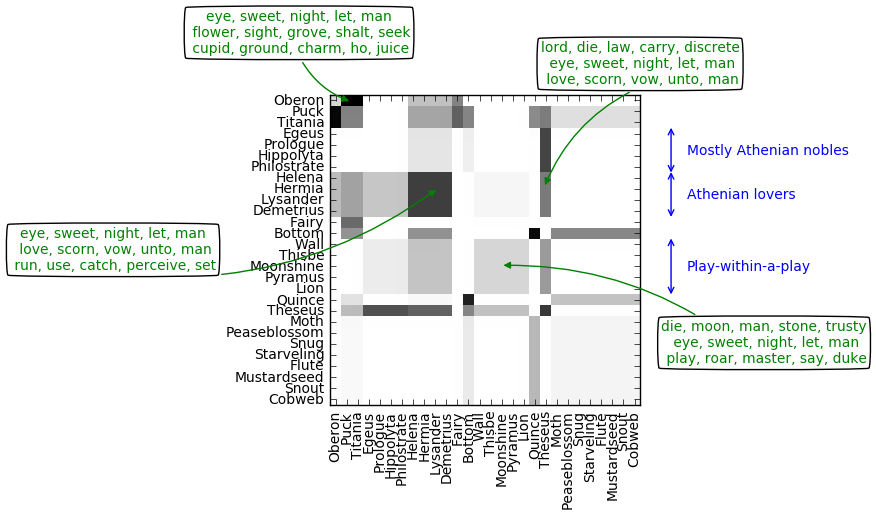
\includegraphics[width=\textwidth]{fig_networktopic/SparseShakeClusters.png}
          \caption{Communities found in ``A  Midsummer Night's Dream'', with highest-probability topics associated with community pairs.}
          \label{fig:shake_topics}
          \end{center}
        \end{figure*}
        
        \begin{figure*}[p]
          \begin{center}
          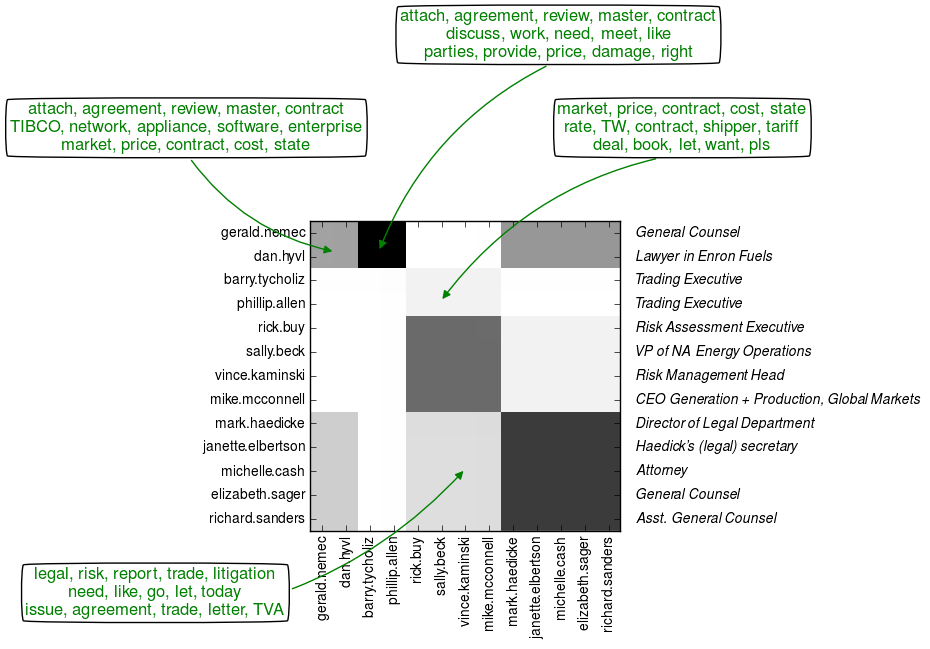
\includegraphics[width=\textwidth]{fig_networktopic/EnronClusters.png}
          \caption{Communities found in the ENRON e-mail corpus for select e-mail participants, with highest-probability topics associated with community pairs.}
          \label{fig:enron_topics}
          \end{center}
        \end{figure*}
        
        \begin{figure*}[p]
          \begin{center}
          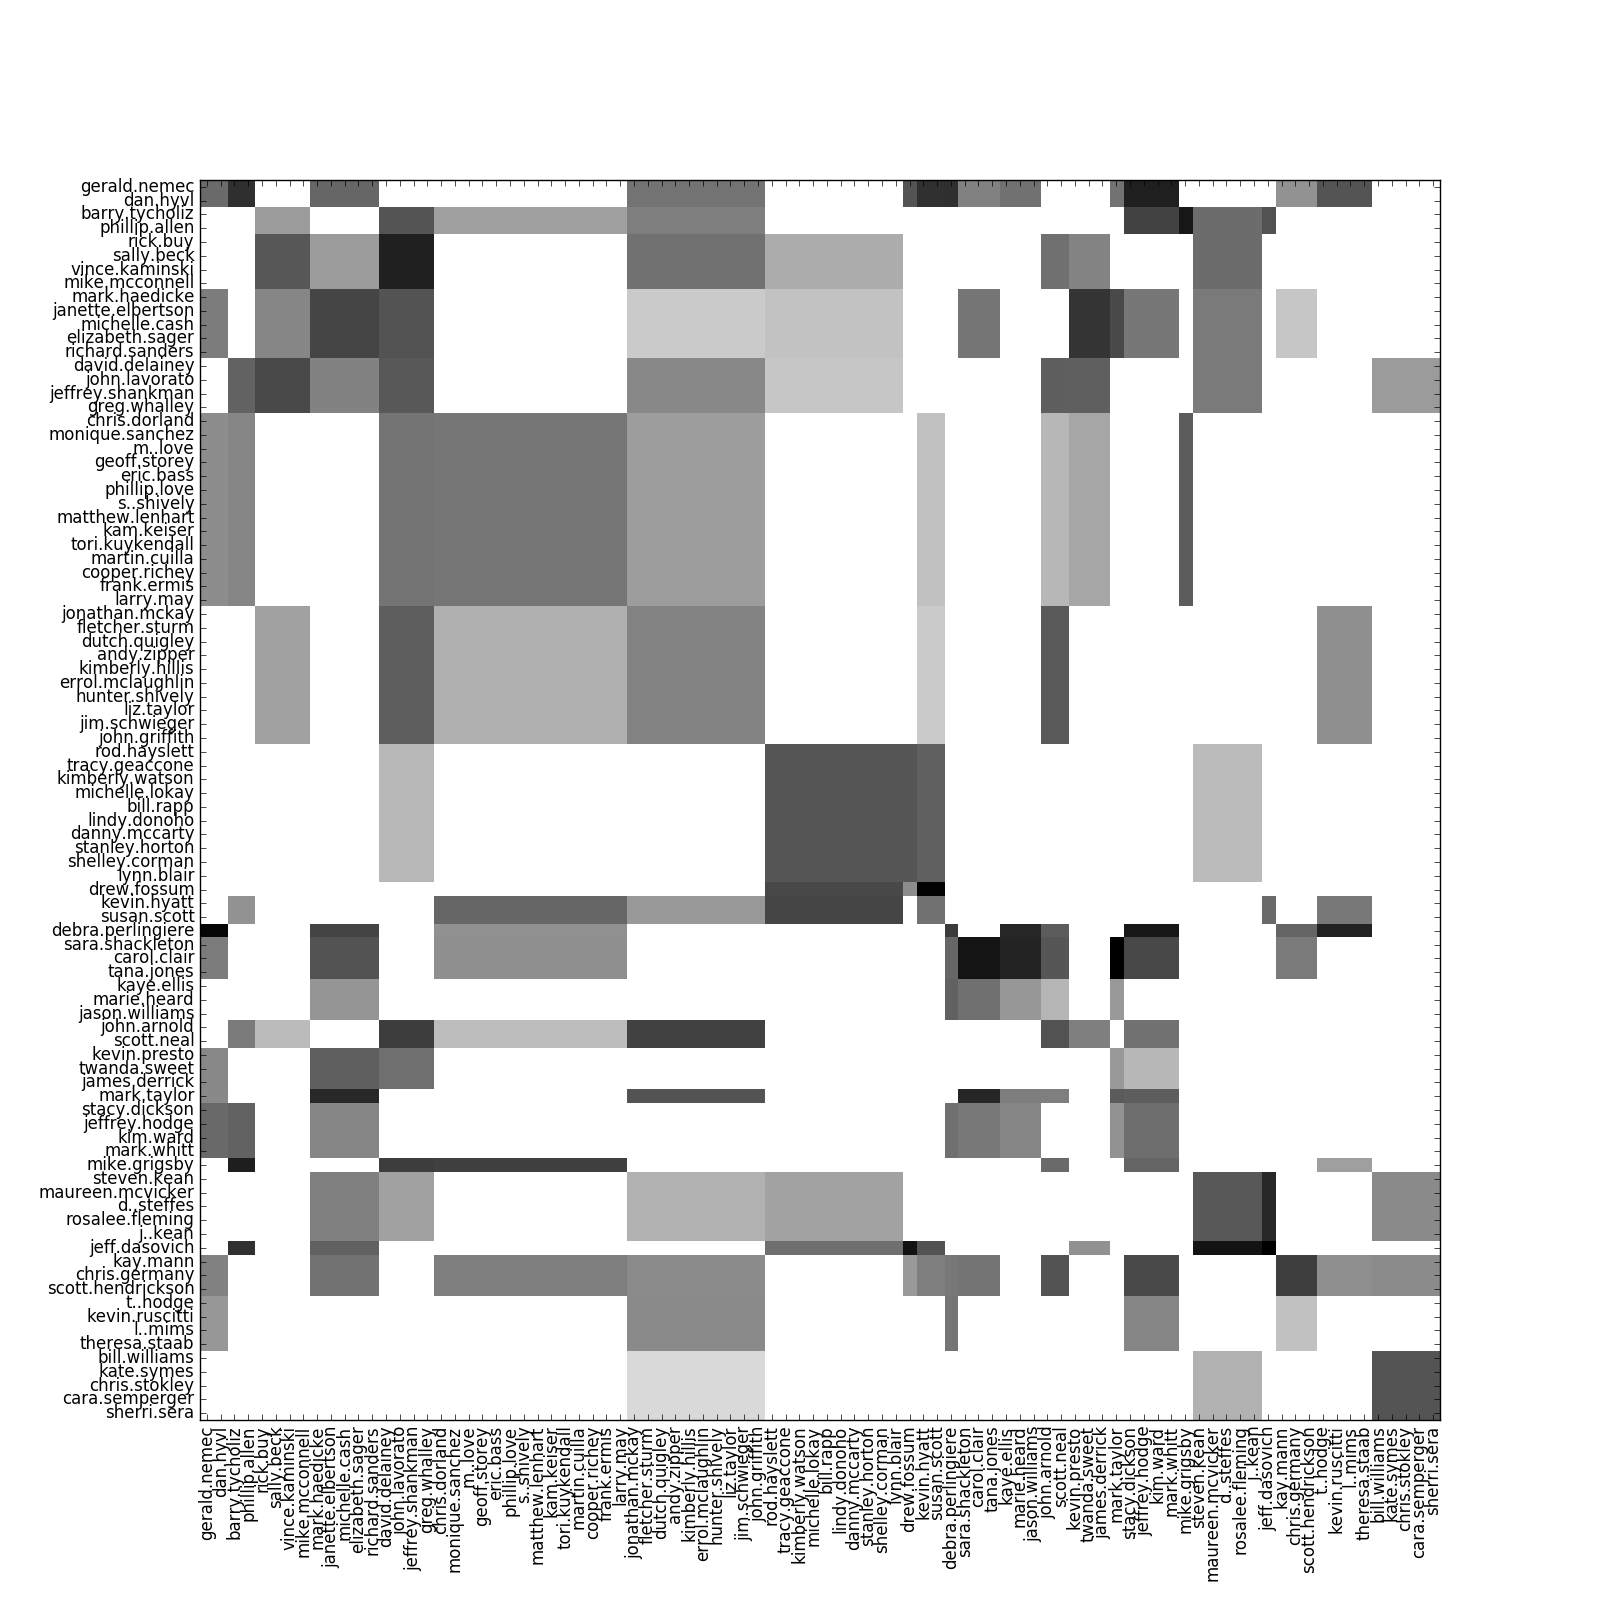
\includegraphics[width=\textwidth]{fig_networktopic/Enron_v2_network_rates.png}
          \caption{Communities found in the ENRON e-mail corpus for all ENRON internal e-mail participants.}
          \label{fig:enron_topics_full}
          \end{center}
        \end{figure*}
    
        We begin with a qualitative analysis of the community structure found using the Topic Blockmodel on ``A Midsummer Night's Dream'', since reader familiarity with the characters allow for easy evaluation of the clusterings found. Figure \ref{fig:shake_topics} shows the community structure obtained using a single sample from the Markov chain (to avoid alignment issues). Here, the shade of  element $(s,r)$ of the matrix represents the gamma random variable $\lambda_{c_s,c_r}^{(\cdot)}$ governing the total number of words sent from node $s$ to node $r$. The community structure can be inferred by looking at the discontinuities: nodes in the same community have the same parameter.
    
        The names of the characters are given on the left hand axis, and some interesting communities are manually annotated on the right. Note that the communities generated are fairly well aligned with the character groupings present in the play.  For example, Demetrius, Helena, Hermia, and Lysander represent a ring of romantically entangled Athenians;  Egeus, Hippolyta and Philostrate are elder Athenian nobility; Wall, Prologue, Thisbe, Moonshine, Pyramus and Lion are all characters in the play-within-a-play; Titania and Puck are both fairies who interact with Oberon in a similar manner. The outliers are mostly characters with very few lines -- for example the minor fairies and the minor mechanicals are intermingled, but all these characters have very few lines.
        
        To demonstrate how the topics characterize the community's relationships, we consider four community-community pairs that discuss love - a major theme of ``A Midsummer Night's Dream''. While all the selected pairs contain a shared topic of romantic words, the additional topics shed nature on the communities' nature. The star-crossed Athenian lovers talk among themselves of love and hate, and talk to Duke Theseus about the consequences of their romantic choices; Oberon talks to Puck and Titania of  magical slumber and fairy mischief; the play-within-a-play characters talk about aspects of the play and appeal to their audience.
        
        Figures \ref{fig:enron_topics} and \ref{fig:enron_topics_full} show the discovered latent social network between a subset of the ENRON employees.  For ease of interpretability, Figure \ref{fig:enron_topics} provides an annotated subset of the Enron employees, their exchanged topics, and the employees' roles in the company; Figure \ref{fig:enron_topics_full} shows the full network. From Figure \ref{fig:enron_topics} we see that attorneys Gerald Nemec and Dan Hyvl are in a community, as are the trading executives Barry Tycholiz and Phillip Allen, as are executives involved in energy development and risk Rick Buy, Sally Beck, Vince Kamisnki, and Mike McConnell.  The fourth community shown is again legal professionals, but with different subject areas.
        
        In the absence of this job title information, one could still use the topics associated with the community-community pairs to improve understanding of the latent network. We see that  the attorneys' emails are focused on agreements and contracts, and supplying advice to the other employees. When the trading executives are talking with the development community, however, they are primarily discussing elements of economic forecasts (market, price, cost, rate, contract, tariff, etc.).  When the second attorney group is writing to the risk group, their topics skew more toward legal risks (e.g. litigation) and government affairs (e.g. dealing with the Tennessee Valley Authority (TVA)) than the contracts advice that the first group of attorneys gives to the trading executives.
    
    \subsection{Quantitative Evaluation}\label{sec:quant}
        We evaluated the predictive performance of the topic blockmodel on four metrics:
        \begin{enumerate}
            \item Log predictive likelihood of the text of held-out documents (conditioned on number of words sent, since this is required for most of the comparison methods). This is designed to mimic the task of predicting the topical content of an email from its sender and recipient.
            \item Log predictive likelihood of the recipient of a held-out email/speech, conditioned on the sender and the text of the communication. This is designed to mimic the task of suggesting recipients for an email.
            \item Log predictive likelihood of the sender and recipient of a held-out email/speech. This is designed to showcase the fact that using the text information allows us to better model latent community structure. 
            \item Log predictive likelihood of the word counts of held-out sender-receiver pairs. This is designed to show that the inclusion of topic information improves count prediction.
        \end{enumerate}
        
        \begin{table}[ht]
        	\caption{Log predictive likelihood ($\pm$ one standard error) of document text, conditioned on sender and recipient where applicable.}
        	\centering
        	\label{tab:topic_prediction}
        	\begin{tabular}{l c c}
        	Model & ENRON &  Shakespeare  \\
        	\noalign{\smallskip}\hline\noalign{\smallskip}
        	LDA	&				-410,110.2 	 $\pm$  50.8	&	--48,716.2	 $\pm$  4.6 \\
        	ART &				-365,600.5 	$\pm$  47.7	&	-47,495.5  $\pm$  4.8 \\
        	CNT	&			-368,983.5 	$\pm$  89.2	&	\textbf{-46,076.6} 	 $\mathbf{\pm}$  \textbf{3.9} \\
        	\textit{Topic Blockmodel}	&				\textbf{-345.632.5} 	$\mathbf{\pm}$  \textbf{4.1}	&	-46,275.9 $\pm$  4.0 \\
        	\noalign{\smallskip}\hline
        	\end{tabular}
        \end{table}
        
        \begin{table}[ht]
        	\caption{Log predictive likelihood ($\pm$ one standard error) of document recipient, conditioned on document content and sender where applicable.}
        	\centering
        	\label{tab:r_prediction}
        	\begin{tabular}{l c c}
        		Model & ENRON &  Shakespeare  \\ 
        		\noalign{\smallskip}\hline\noalign{\smallskip}
        		ART				& -204,585.3		$\pm$  6.4		&	-19,809.7 	$\pm$  1.1 \\
        		CNT			& -216,278.9		$\pm$   $<$0.1		&	-19,703.3 	$\pm$  $<$0.1 \\
        		 Poisson-SBM				& -160,984.7		$\pm$  148.6	&	-14,587.2	$\pm$  35.9 \\
        		\textit{Topic Blockmodel}			& \textbf{-137,199.8} $\mathbf{\pm}$  \textbf{53.2}	&	\textbf{-12,997.8} 	 $\mathbf{\pm}$  \textbf{20.6} \\
        	\noalign{\smallskip}\hline
        	\end{tabular}
        \end{table}
    
        \begin{table}[ht]
        	\caption{Log predictive likelihood ($\pm$ one standard error) of document sender and recipient, conditioned on document content where applicable.}
        	\centering
        	\label{tab:sr_prediction}
        	\begin{tabular}{l c c}
        		Model & ENRON &  Shakespeare   \\
        		\noalign{\smallskip}\hline\noalign{\smallskip}
        		ART				& -416,588.6		$\pm$  6.8		&	-39,580.0 	$\pm$  1.0 \\
        		CNT				& -432,557.7		$\pm$   $<$0.1		&	-39,406.7 	$\pm$  $<$0.1 \\
        		 Poisson-SBM			& -347,479.6		$\pm$  148.6	&	-31,400.3 	$\pm$  35.9 \\
        		\textit{Topic Blockmodel}			& \textbf{-321,127.8} 	$\mathbf{\pm}$  \textbf{53.3}	&	\textbf{-29,614.0} 	 $\mathbf{\pm}$  \textbf{20.6} \\
        	\noalign{\smallskip}\hline
        	\end{tabular}
        \end{table}
        
        \begin{table}[ht]
        	\caption{Log predictive likelihood ($\pm$ one standard error) of sender and recipient counts.}
        	\centering
        	\label{tab:count_prediction}
        	\begin{tabular}{l c c}
        		Model & ENRON &  Shakespeare   \\
        		\noalign{\smallskip}\hline\noalign{\smallskip}
        		 Poisson-SBM			& -92,851.2		$\pm$  12.1	&	-103,411.4 	$\pm$  0.6 \\
        		\textit{Topic Blockmodel}			& \textbf{-88,730.4} 	$\mathbf{\pm}$  \textbf{3.1}	&	\textbf{-102,549.8} 	 $\mathbf{\pm}$  \textbf{0.2} \\
        	\noalign{\smallskip}\hline
        	\end{tabular}
        \end{table}

    \subsubsection{Log-likelihood of words in held-out documents}
    
        For the first task, we randomly held out 10\% of documents, and evaluated the predictive log likelihood of this test set using the  comparison models with a topic model component (i.e.\ LDA, ART, and CNT). The log predictive likelihoods are shown in Table \ref{tab:topic_prediction}. 
    
        We see that the Topic Blockmodel performs significantly better than the competitors on the ENRON dataset. In this realistic setting, the number of emails sent between two individuals is highly indicative of their relationship, so we see a significant advantage from jointly modeling the number of words and their content. In particular, we see that the Topic Blockmodel outperforms our Clustered Node Topic Model variant, which does not model counts and treats zero edges as missing.
        
        On the Shakespeare data, the Topic Blockmodel performs slightly worse than the Clustered-Node Topic model, though still better than LDA or ART. We believe that this is due to the artificial nature of the network. The community structure in ``A Midsummer Night's Dream'' is man-made, and designed so that the many separate communities interact in complex, artful manners. Moreover, by assuming a speech is directed to (only) the previous speaker, we are working with a noisy approximation to Shakespeare's intended interaction network.  Since the Clustered-Node Topic Model does not model the number of links, it will be less hampered by an unrealistic network structure. 
        
    \subsubsection{Recipient Attribution}

        For the second task, designed to mimic automatic email recipient suggestion, we again held out 10\% of documents and  predicted the recipient of each document based on the document's length, text and sender. 
        We compared against the three comparison methods with a network component, namely ART, CNT, and the Poisson Stochastic Blockmodel. Prediction in ART and CNT does not take into account the number of words sent; prediction in the Poisson Stochastic Blockmodel does not take into account the specific words sent. Table \ref{tab:r_prediction} shows the test set log predictive likelihood for the four methods on the recipient attribution task.
        
        In the ENRON e-mail data, we again see that the Topic Blockmodel performs significantly better than any of the competitive models in identifying the correct sender-recipient pair, with the Poisson Stochastic Blockmodel coming  second and the two models that do not consider word counts performing worst. The relative performance of the Poisson Stochastic Blockmodel (which does not consider topic distributions) versus CNT and ART (which do not consider word counts) suggests that count modeling, rather than topic modeling, is the more important component in this setting; however by combining these two components the Topic Blockmodel is able to make use of the topic distribution to improve prediction over the purely count-based model.
        
        We see a similar pattern in the Shakespeare data: the Topic Blockmodel  outperforms the Poisson Stochastic Blockmodel and all other models, and the models that just consider topical content of documents perform worse than the Poisson Stochastic Blockmodel that only considers counts.  This is again likely for similar reasons to ENRON: the models on interaction intensity are able to down-weight pairs that very rarely interact, greatly boosting the likelihood of pairs that are expected to interact, and further identifying the correct topic mixture within high-intensity community pairings.

    \subsubsection{Sender/Recipient Attribution}
    
        For the third task, we again held out 10\% of documents and  predicted both sender and recipient based on a document's length and text, comparing against ART, CNT and the Poisson Stochastic Blockmodel. The resulting log predictive likelihoods, shown in Table \ref{tab:sr_prediction}, tell a similar story to the sender attribution task: the Poisson Stochastic Blockmodel, which only considers document length, outperforms CNT and ART which only consider document text, suggesting document length is more important than document semantic content in this task. However, the Topic Blockmodel, by making use of both length and semantic content, is able to outperform all three comparison methods on both tasks.
    
    \subsubsection{Edge Count Prediction}
    
        Finally, we withheld 10\% of sender-receiver pairs in the network and predicted the word count of the withheld links based on the assigned communities of the sender and receiver.  Table \ref{tab:count_prediction} shows that, in both the ENRON and Shakespeare data sets, the Topic Blockmodel significantly improves on the Poisson Stochastic Blockmodel, which is the only comparison model discussed which models the word counts of heldout links.
    
\section{Discussion and Future Work}\label{sec:conclusion}
    
    In this work we introduced a unified network and topic model, the Topic Blockmodel. Inspired by existing stand-alone network and topic models, the Topic Blockmodel can be used to identify and label communities in a network and make predictions about interactions. %In human-generated data, the model performs better than existing methods at prediction of heldout message information and attribution of messages.
    
    We have focused here on networks where the interactions are textual in nature. However, we may also have networks where interactions take the form of images, audio, or some combination of media. A future research direction might be to explore augmenting this model with other forms of media to better make use of information shared across the network, using likelihoods such as those described in \citep{cao2007spatially}, \citep{niu2012context} or \citep{kim2009acoustic}.
    
    Other extensions could be obtained by using a richer distribution over the community structure. We chose a simple, parametric model with single-community membership to allow for straightforward computation; however the potential for mixed-membership or nonparametric versions is clear. Another interesting avenue for research is to make the distribution over communities explicitly dependent on some set of covariates such as time of email or geographical location of nodes, creating a dynamic model.

    One limitation of the stochastic blockmodel framework is that it is only appropriate when our network is dense -- that is, when the number of non-zero edges grows quadratically with the number of nodes. This is a reasonable assumption in relatively small networks where it is likely that all nodes have had a chance to interact with each other -- for example, groups of individuals within a school, company or organization, as we have explored in this work.
    
    An interesting parallel line of research, which we are currently exploring, is models for text-based interaction in \textit{sparse} data. Such a model would require replacing the stochastic blockmodel component of the model with a distribution appropriate for sparse graphs, such as those described by \citep{Caron:Fox:2014}, \citep{Veitch:Roy:2015}, \citep{Cai:Campbell:Broderick:2016}, \citep{Crane:Dempsey:2016} and \citep{williamson2016nonparametric}. Without such a significant change to the model, one possible direction would be to add node-specific degree-correcting parameters as proposed by \citep{Karrer:Newman:2011}.

    %This model has several possible extensions that will be considered in future work: a mixed membership model \cite[similar to ][]{mccallum2007topic}, an infinite-dimensional hierarchical topic model \cite[see ][]{teh2004sharing}, and inclusion of other rich data such as images or sounds \cite[related methods include ][]{cao2007spatially,niu2012context,kim2009acoustic}. These extensions expand not only the model structure but the richness of edge information and therefore variety of networks on which it is applicable.


\chapter{Monotonic Fairness}

\section{one section}

blah blah blah

\chapter{Elicited Monotonic Fairness}
\label{ch:SoftMonoFair}

\section{Overview}

    Monotonicity as discussed in Chapter \ref{ch:MonoFair} requires that individual attributes can be assigned a monotonic relationship with the outcome, but does not account for intuitive monotonicity which might occur across combinations of attributes.  

\section{Background}\label{sec:softmono_bg}
    
    We assume that the reader is familiar with the definitions and concepts in Sections \ref{sec:monofair_intro} and \ref{sec:monofair_background}.
    
    Topics to cover:
    \begin{itemize}
        \item Survey methodologies for eliciting rankings
        \item Learning ranking functions
        \item Recent ML fairness works that deal with elicited fairness
    \end{itemize}
    
    \subsection{Eliciting relationships}
    
    \subsection{Preference Learning}
    
    \subsection{Recent relevant works}
    
\section{Model}\label{sec:softmono_model}

    

\section{Experiments}\label{sec:softmono_experiments}

    

\section{Results}\label{sec:softmono_results}
    

\section{Discussion}\label{sec:softmono_discussion}


%\chapter{Making Tables and Including Figures}
\index{Making Tables and Including Figures@\emph{Making Tables
	and Including Figures}}%

The \emph{tabular} 
\index{commands!environments!tabular}%
environment allows us to create complex 
tables and figures, and draw boundaries around and within it.
The following example illustrates this:

\begin{table}[h]
\begin{center}
\caption{An example of a table.}
\vskip 10pt
\begin{tabular}{|ll|l|ll|l|lll|}
\cline{1-2} \cline{4-5} \cline{7-9}
\multicolumn{2}{|c|} {\textsl{Gegenwart}} & &
\multicolumn{2}{|c|} {\textsl{Imperfekt}} & &
\multicolumn{3}{|c|} {\textsl{Perfekt}} \\
\cline{1-2} \cline{4-5} \cline{7-9}
ich & bin  & & ich & war   & & ich & bin  & gewesen \\
du  & bist & & du  & warst & & du  & bist & gewesen \\
er  &      & & er  &       & & er  &      &         \\
sie & ist  & & sie & wart  & & sie & ist  & gewesen \\
es  &      & & es  &       & & es  &      &         \\
\cline{1-2} \cline{4-5} \cline{7-9}
wir & sind & & wir & waren & & wir & sind & gewesen \\
ihr & seid & & ihr & wart  & & ihr & seid & gewesen \\
sie & sind & & sie & waren & & sie & sind & gewesen \\
\cline{1-2} \cline{4-5} \cline{7-9}
Sie & sind & & Sie & waren & & Sie & sind & gewesen \\
\cline{1-2} \cline{4-5} \cline{7-9}
\end{tabular} \\[10pt]
Note: The assistance of Herr Professor Lothar Frommhold \\
in generating this table of German declensions \\
is gratefully acknowledged.
\vskip -20pt
\end{center}
\end{table}
\index{commands!environments!table}%

This table was created with the following sequence 
of commands:
\begin{verbatim}
\begin{table}[h]
\begin{center}
\caption{An example of a table.}
\vskip 10pt
\begin{tabular}{|ll|l|ll|l|lll|}
\cline{1-2} \cline{4-5} \cline{7-9}
\multicolumn{2}{|c|} {\textsl{Gegenwart}} & &
\multicolumn{2}{|c|} {\textsl{Imperfekt}} & &
\multicolumn{3}{|c|} {\textsl{Perfekt}} \\
\cline{1-2} \cline{4-5} \cline{7-9}
ich & bin  & & ich & war   & & ich & bin  & gewesen \\
du  & bist & & du  & warst & & du  & bist & gewesen \\
er  &      & & er  &       & & er  &      &         \\
sie & ist  & & sie & wart  & & sie & ist  & gewesen \\
es  &      & & es  &       & & es  &      &         \\
\cline{1-2} \cline{4-5} \cline{7-9}
wir & sind & & wir & waren & & wir & sind & gewesen \\
ihr & seid & & ihr & wart  & & ihr & seid & gewesen \\
sie & sind & & sie & waren & & sie & sind & gewesen \\
\cline{1-2} \cline{4-5} \cline{7-9}
Sie & sind & & Sie & waren & & Sie & sind & gewesen \\
\cline{1-2} \cline{4-5} \cline{7-9}
\end{tabular} \\[10pt]
Note: The assistance of Herr Professor Lothar Frommhold \\
in generating this table of German declensions \\
is gratefully acknowledged.
\vskip -20pt
\end{center}
\end{table}
\index{commands!environments!table}%
\end{verbatim}

The argument \texttt{h} indicates the position for the 
table, in this case ``here if possible''. Other values
of this argument are:
\texttt{t} (top of the page),
\texttt{b} (bottom of the page),
\texttt{p} (on the page of floats) and 
\texttt{H} (HERE! - requires using the package float.sty.
Note: When this option is used, LaTeX ignores all of its formatting
rules and does what you say, putting the entire float exactly where
it is defined. Check your output to make sure it is what you want!
If you are having trouble with LaTeX wanting to put a figure that's
larger than roughly half-a-page, as well as all of the figures
following it, at the end of a chapter, try using the command
\cn{clearpage} immediately following the large figure --- and maybe
a \cn{newpage} later.)
It is possible to combine several arguments, such as
\texttt{ht} (``here if possible, otherwise on top of
the page''). The default is \texttt{tbp}.

Figure \ref{f:ex} is a typical example of inclusion of a 
figure contained in an encapsulated PostScript file. 
\index{PostScript}%
\index{encapsulated PostScript}%
In order to use it, it is necessary to include the 
command \cn{usepackage\{psfig\}} 
\index{psfig}%
at the beginning of the document.

\begin{figure}[htb] % Imported eps example.
\begin{center}
\ 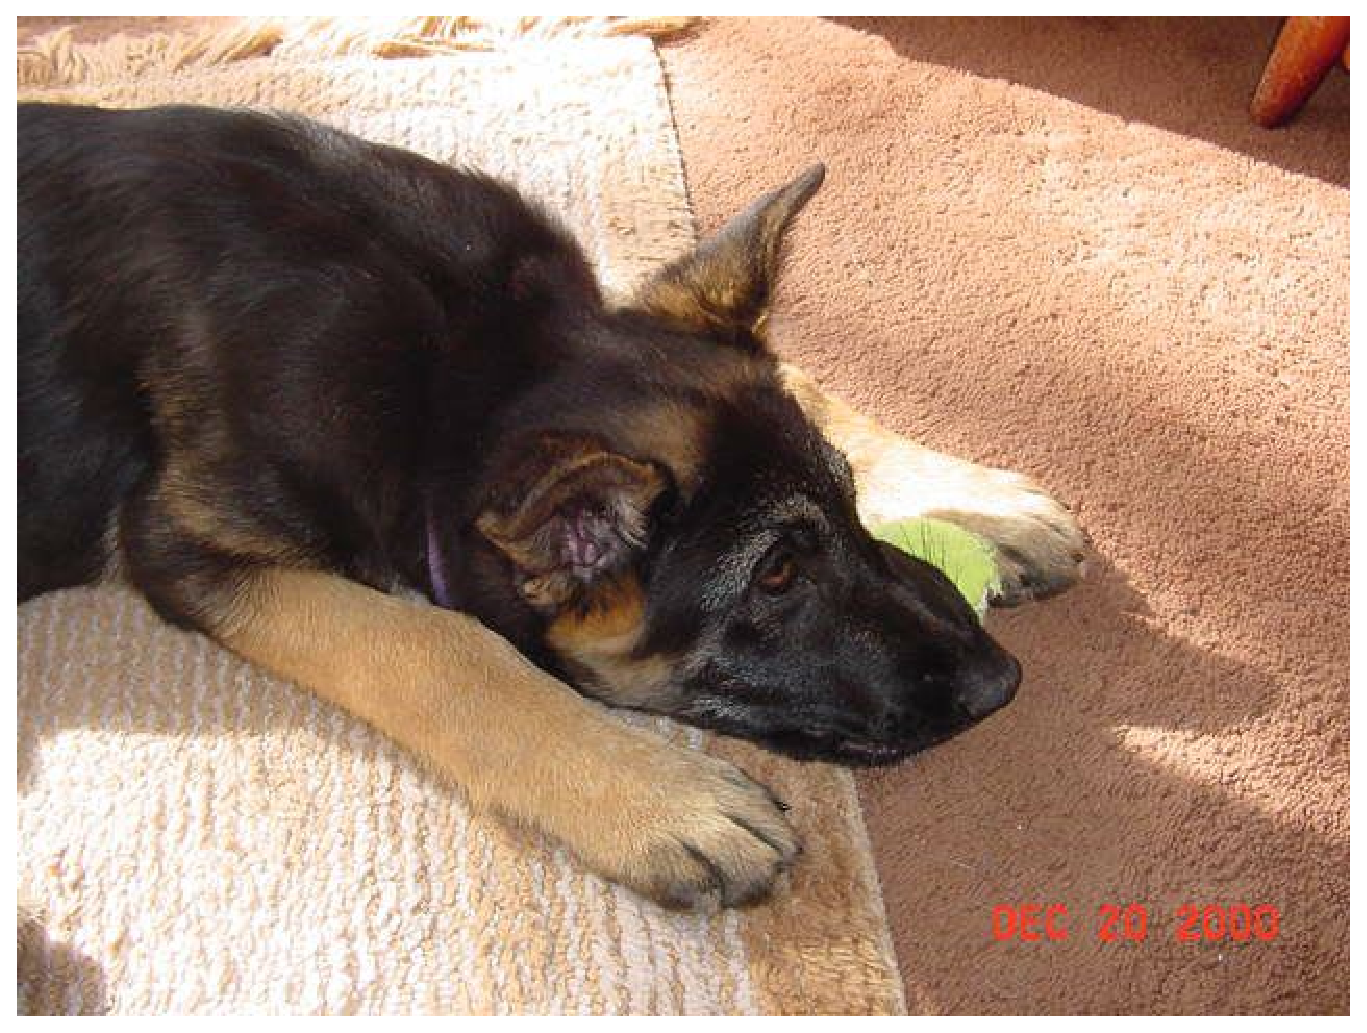
\psfig{file=pup-on-rug.eps,height=1.5in,width=2.0in}
\caption{An example of an imported eps file.}
\label{f:ex}
\end{center}
\end{figure}
\index{commands!environments!figure}%
You can see the commands that generated this
figure in the source file. Look for the line
\cn{begin\{figure\}[htb] \% Imported eps example. }

The command that imports the file is \cn{psfig}, and it also 
controls its size (\texttt{height} and \texttt{width}), and 
can rotate the figure (\texttt{angle}).

Figures can also be drawn by using \LaTeX{} commands. 
Figure \ref{f:circuit} is an example 
(taken from \cite{gms:tlc}).

\begin{figure}[htb] % Picture example.
\begin{center}
   \setlength{\unitlength}{4mm}
   \begin{picture}(12,10)(-2,0)
      \linethickness{0.4pt}
      \qbezier(2.00,6.00)(7.00,6.00)(9.00,3.00)
      \qbezier(2.00,0.00)(7.00,0.00)(9.00,3.00)
      \qbezier(2.00,6.00)(4.00,3.00)(2.00,0.00)
      \qbezier(1.00,6.00)(3.00,3.00)(1.00,0.00)
      \put(9.75,3.00){\circle{1.50}}
      \put(10.50,3.00){\line(1,0){1.50}}
      \put(0.00,5.00){\line(1,0){1.50}}
      \put(0.00,1.00){\line(1,0){1.50}}
   \end{picture}
\caption{An example of a picture}
\label{f:circuit}
\end{center}
\end{figure}
\index{picture}%

The commands that generated this
picture are in the source file following the line
\cn{begin\{figure\}[htb] \% Picture example.  }

The commands used have rather obvious meanings. In particular, 
the command \cn{qbezier} 
\index{commands!qbezier@\cn{qbezier}}%
draws a quadratic Bezier curve, 
defined by its two ending points, and a third point (whose 
coordinates are in the middle) that is used as control point. 
Figure \ref{f:qb} illustrates the effect of the control point:

%\begin{figure}[htb] % Bezier curves example.
\begin{figure}[h] % Bezier curves example.
\begin{center}
   \setlength{\unitlength}{.8mm}
   \begin{picture}(55,55)(-15,0)
      \linethickness{1pt}
      \qbezier(0,0)(-10,30)(50,30)
      \qbezier(0,0)(20,50)(50,30)
      \thinlines
      \put(0,0){\line(-1,3){10}}
      \put(50,30){\line(-1,0){60}}
      \put(0,0){\line(2,5){20}}
      \put(50,30){\line(-3,2){30}}
      \put(0,0){\circle*{1}}
      \put(0,-1){\makebox(0,0)[t]{$A_{0,0}$}}
      \put(-10,30){\circle*{1}}
      \put(-10,31){\makebox(0,0)[b]{$B_{10,30}$}}
      \put(50,30){\circle*{1}}
      \put(58,29){\makebox(0,0)[b]{$C_{50,30}$}}
      \put(20,50){\circle*{1}}
      \put(20,51){\makebox(0,0)[b]{$D_{20,50}$}}
   \end{picture}
\caption{Bezier curves}
\label{f:qb}
\end{center}
\end{figure}
\index{Bezier curves}%


This figure has been generated with the following commands:
\begin{verbatim}
\begin{figure}[htb] % Bezier curves example.
\begin{center}
   \setlength{\unitlength}{.8mm}
   \begin{picture}(55,55)(-15,0)
      \linethickness{1pt}
      \qbezier(0,0)(-10,30)(50,30)
      \qbezier(0,0)(20,50)(50,30)
      \thinlines
      \put(0,0){\line(-1,3){10}}
      \put(50,30){\line(-1,0){60}}
      \put(0,0){\line(2,5){20}}
      \put(50,30){\line(-3,2){30}}
      \put(0,0){\circle*{1}}
      \put(0,-1){\makebox(0,0)[t]{$A_{0,0}$}}
      \put(-10,30){\circle*{1}}
      \put(-10,31){\makebox(0,0)[b]{$B_{10,30}$}}
      \put(50,30){\circle*{1}}
      \put(58,29){\makebox(0,0)[b]{$C_{50,30}$}}
      \put(20,50){\circle*{1}}
      \put(20,51){\makebox(0,0)[b]{$D_{20,50}$}}
   \end{picture}
\caption{Bezier curves}
\label{f:qb}
\end{center}
\end{figure}
\end{verbatim}



%\chapter{An Example of Mathematical Writing}
\index{An Example of Mathematical Writing%
@\emph{An Example of Mathematical Writing}}%

\section{Generalized Fatou's Lemma}
\index{Generalized Fatou's Lemma%
@\emph{Generalized Fatou's Lemma}}%

Here we show an application of the following lemma:

\begin{lem}[Generalized Fatou's Lemma] \label{l:fatou}

Let $A$ be a Dedekind ring and $F$ a rational series 
in $A[[X]]$, i.e., $F = p/q$ for some 
$p, q \in A[X]$. Then there exist two polynomials 
$P, Q \in A[X]$ such that $F = P/Q$, 
where $P$ and $Q$ are relatively prime and 
$Q(0) = 1$.

\end{lem}

\proof
See \cite{bertin:psn}, p.~15, theorem~1.3.
\endproof

\begin{thm} \label{l:req}
Let $\{c_n\}_{n=-\infty}^{\infty}$ a set of 
elements from $K$ such that $c_n \in k'$ for every 
$n \geq n_0$, and verifying the following recurrence 
relation of order M:
\begin{equation}
c_n\ =\ r_1\,c_{n-1} + r_2\,c_{n-2} + \dots + r_M\,c_{n-M}
\end{equation}
for every $n \in \mathbb Z$, where $r_1,r_2,\dots,r_M$ are in 
$K$, $r_M \neq 0$. 
Then:

\item{(i)} The coefficients $r_1,r_2,\dots,r_M$ are in 
$k'$, and for every $n \in \mathbb Z$, $c_n \in k'$.

\item{(ii)} If $c_n \in \mathcal O_{k',v}$ 
for every $n \geq n_0$, then the coefficients 
$r_1,r_2,\dots,r_M$ are all in 
$\mathcal O_{k',v}$.

\end{thm}


\proof 

\item{(i)} Let $C_n$ and $R$ be the matrices:

\begin{equation}
C_n\ =
\ \left(
\begin{array}{llll}
              c_n & c_{n+1} & \hdots & c_{n+M-1} \\
              c_{n+1} & c_{n+2} & \hdots  & c_{n+M} \\
              \vdots & \vdots & \ddots & \vdots \\
              c_{n+M-1} & c_{n+M} & \hdots & c_{n+2M-2}
\end{array}
\right)
\end{equation}
and
\begin{equation}
R\ =
\ \left(
\begin{array}{lllll}
              0 & 1 & 0 & \hdots & 0 \\
              0 & 0 & 1 & \hdots & 0 \\
             \vdots & \vdots & \vdots & \ddots & \vdots \\
              0 & 0 & 0 & \hdots & 1 \\
              r_M & r_{M-1} & r_{M-2} & \hdots & r_1 
\end{array}
\right)
\end{equation} 

We have that $C_{n+1} = R\,C_n$. Since the recurrence 
relation is of order M, $C_n$ is non singular. 
On the other hand, $R = C_{n+1}\,C_{n}^{-1}$. Since the 
elements of $C_n$ are in $k'$ for $n \geq n_0$, the entries 
of $R$, and those of $R^{-1}$, will be in $k'$. Since 
$C_{n-1} = R^{-1}\,C_n$, we get that the entries of 
$C_n$ will be in $k'$ also for $n < n_0$. 

\item{(ii)} For each $t \geq n_0$ define the formal 
power series 

\begin{equation}
F_t(X)\ =\ \sum_{n=0}^{\infty} c_{t+n}\,X^n
\end{equation}
which is in $\mathcal O_{k',v}[[X]]$. 
We have $F_t(X) = p_t(X)/q(X)$, 
where $p_t(X),q(X) \in k'[X]$ are the following:
\begin{equation}
p_t(X)\ =\ \sum_{j=0}^{M-1} \Bigl( c_{t+j} - 
                    \sum_{i=1}^{j} r_i\,c_{t+j-i} \Bigr)\,X^j
\end{equation}
\begin{equation}
q(X)\ =\ 1 - r_1\,X - r_2\,X^2 - \dots - r_M\,X^M
\end{equation}
This can be checked by multiplying $F_t(X)$ by $q_t(X)$ 
and using the recurrence relation, which gives 
$F_t(X)\,q(X) = p_t(X)$ (see \cite{poorten:sp}). 

Now we will prove that $p_t(X)$ and $q(X)$ are relatively 
prime. To do so, we will see that they cannot have any 
common root (in $\overline {k'}$). In fact, assume 
that $\alpha$ is a common root of $p_{t_0}(X)$ and $q(X)$ 
for some $t_0 \geq n_0$, i.e.: 
$p_{t_0}(\alpha) = q(\alpha) = 0$. 
Since $q(0)=1$, then $\alpha \neq 0$. Now we have:
\begin{equation}
X\,F_{t_0+1}(X) = F_{t_0}(X) - c_{t_0}
\end{equation}
so:
\begin{multline}
X\,p_{t_0+1}(X) = X\,q(X)\,F_{t_0+1}(X) \\
= q(X)\,(F_{t_0}(X) - c_{t_0}) = p_{t_0}(X) - c_{t_0}\,q(X)
\end{multline}
Hence $p_{t_0+1}(\alpha) = 0$, which means that $\alpha$ is 
also a root of $p_{t_0+1}(X)$. By induction we get that 
$p_t(\alpha) = 0$ for every $t \geq t_0$. Grouping the 
terms of $p_t(X)$ with respect to $c_t,c_{t+1},\dots,c_{t+M-1}$, 
we get:
\begin{equation}
p_t(X) = \sum_{j=0}^{M-1} a_j(X)\,c_{t+j}
\end{equation}
where 
\begin{equation}
a_j(X) = X^j\,\Bigl( 1 - \sum_{i=1}^{M-j-1} r_i\,X^i \Bigr)
\end{equation}
Note that $a_0(X),a_1(X),\dots,a_{M-1}(X)$ do not depend on t. 
On the other hand $p_t(\alpha)=0$ implies
\begin{equation}
\label{e:coldep}
\sum_{j=0}^{M-1} a_j(\alpha)\,c_{t+j} = 0
\end{equation}
for every $t \geq t_0$. Note that $a_{M-1}(\alpha)=\alpha^{M-1}
\neq 0$, so $a_0(\alpha),a_1(\alpha),\dots,a_{M-1}(\alpha)$ 
are not all zero, and (\ref{e:coldep}) means that the columns 
of the matrix $C_{t_0}$ are linearly dependent, so 
$\det C_{t_0}=0$, which contradicts the fact that $C_{t_0}$ 
is non singular. Hence, the hypothesis that $p_t(X)$ and 
$q(X)$ have a common root has to be false. This proves that 
$p_t(X)$ and $q(X)$ are relatively prime. 

By (generalized Fatou's) lemma~\ref{l:fatou}, 
and taking into account that 
$\mathcal O_{k',v}$ is a Dedekind ring, 
we get that there exist two relatively prime 
polynomials $P_t(X)$ and $Q_t(X)$ in 
$\mathcal O_{k',v}[X]$ such that 
$F_t(X) = P_t(X)/Q_t(X)$ and $Q_t(0)=1$. Hence: 
$p_t(X)\,Q_t(X) = q(X)\,P_t(X)$. By unique factorization 
of polynomials in $k'[X]$, there is a $u \in k'$ such that 
$P_t(X) = u\,p_t(X)$ and $Q_t(X) = u\,q_t(X)$. Since 
$Q_t(0)=q(0)=1$, we get that $u=1$, so 
$P_t(X) = p_t(X)$ and $Q_t(X) = q(X)$. 
Hence, the coefficients of $q(X)$ are in 
$\mathcal O_{k',v}$. 

\endproof


\section{Other Examples of Mathematical Writing}

\subsection{An Example of a Commutative Diagram}
\index{An Example of a Commutative Diagram%
@{An Example of a Commutative Diagram}}%

The following is an example of a commutative diagram.
\index{commutative diagram}%
It requires the \texttt{amscd} package.
\index{amscd package@{\texttt{amscd} package}}

\begin{equation*}
\newcommand{\End}{\operatorname{End}}
\begin{CD}
S^{{\mathcal{W}}_\Lambda}\otimes T   @>j>>   T\\
@VVV                                    @VV{\End P}V\\
(S\otimes T)/I                  @=      (Z\otimes T)/J
\end{CD}
\end{equation*}

That diagram has been made with the following commands:

\begin{verbatim}
\newcommand{\End}{\operatorname{End}}
\begin{CD}
S^{{\mathcal{W}}_\Lambda}\otimes T   @>j>>   T\\
@VVV                                    @VV{\End P}V\\
(S\otimes T)/I                  @=      (Z\otimes T)/J
\end{CD}
\end{verbatim}

\subsection{Using AMS Fonts}
\index{Using AMS Fonts@{Using AMS Fonts}}

To use AMS fonts it is necessary to choose from an assortment 
of \LaTeX{} packages. For instance the command 
\cn{usepackage\{amsfonts\}} calls in the \emph{amsfonts} package, 
which provides blackboard bold letters (e.g. $\mathbb{R}$) and 
some math symbols. A superset of that package is 
\emph{amssymb}. Other packages are \emph{eufrak} 
for Frankfurt letters (e.g. $\mathfrak{R}$)
and \emph{eucal} for Euler script 
(e.g. $\mathcal{R}$). 
Consult the \LaTeX{} documentation about this subject 
for additional information.



%%%%%%%%%%%%%%%%%%%%%%%%%%%%%%%%%%%%%%%%%%%%%%%%%%%%%%%%%%%%%%%%%%%%%%
% Appendix/Appendices                                                %
%%%%%%%%%%%%%%%%%%%%%%%%%%%%%%%%%%%%%%%%%%%%%%%%%%%%%%%%%%%%%%%%%%%%%%
%
% If you have only one appendix, use the command \appendix instead
% of \appendices.
%
\appendices
\index{Appendices@\emph{Appendices}}%


\chapter{Appendix: Monotonic Fairness Supplement}

In this supplement, we provide justification for our design choices for the neural network architecture, and demonstrate that such an architecture is able to capture monotonic functions, and impose monotonicity even when the true generating function is non-monotone.

\section{Design choices}
    Below, we discuss several design choices, and their effect on the resulting functions.

    \paragraph{Transformation Matters:} 
        The choice of transformation function in Equation 4 can have a significant effect on the probability of successful convergence of monotonic neural networks.  We show in Figure~\ref{fig:activations} that the choice of transformation can have different effects based on the nature of the underlying function, and affects both monotonic and non-monotonic fitting. We consider four non-linearities:
        \begin{itemize}
            \item Square: $\tau(x) = x^2$.
            \item Abs: $\tau(x) = |x|$.
            \item Offset exponential linear unit (elumod): \\$ \tau(x) = \left\{\begin{array}{c l} 
                    x       & ~\mbox{if}~ x > 1 \\ 
                    e^{x-1} & ~\mbox{if}~ x \le 1 \\ 
                \end{array}\right.$
            \item Softplus: $\tau(x) = \log(1+e^x)$
        \end{itemize}
        We choose to use an offset exponential linear unit in our experiments, since it achieved optimal or near-optimal convergence in these comparisons.
        
        \begin{figure}
            \centering
            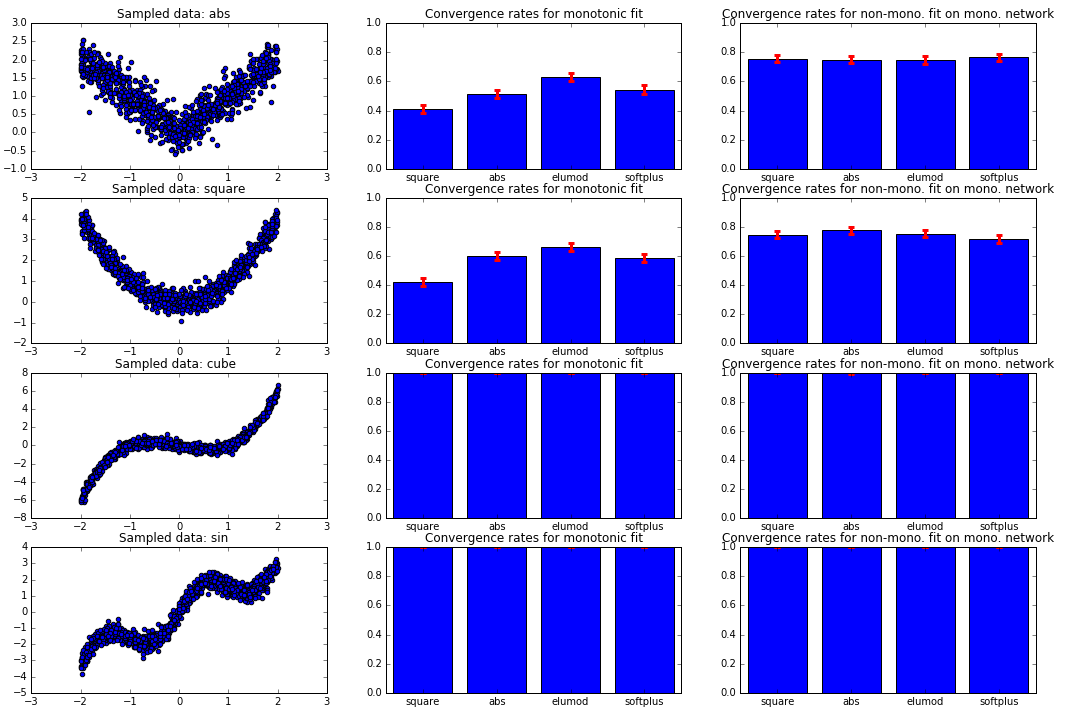
\includegraphics[width=\textwidth]{fig_monofair/activation_function_convergence.png}
            \caption{Convergence rates for various functions used to enforce positive weights. The vertical exist for the middle and right columns is the proportion of random initialization which converge to a non-deviant ($\hat{y} = \bar{y}$) solution.}
            \label{fig:activations}
        \end{figure}

    \paragraph{Activation Matters:} 
        Additional caution is needed in selecting an activation function for a monotonic neural network.  If, for instance, a convex activation function is used (e.g. \textit{elu} or \textit{relu}), subsequent layers can only compound this convexity, and the resulting function can only be convex.  It is easy to see this by considering the compounding of the first and second derivative across the layers.  This may be a desirable feature in some settings, but generally prohibits it from approximating \textit{any} monotonic function.  As such, bounded (but monotonic) activation functions like \textit{logistic} or \textit{tanh} are advisable for general purposes.
    
\section{Ability to Capture Mixed Monotonicity}

    We wish to emphasize that the network architecture described in this paper can simultaneously handle monotonic and non-monotonic relationships between the inputs and output. If we begin with the assumption that a network constrained to positive weights will produce a monotonically increasing function $f(x)$, we can briefly intuit the ability to fit a monotonically decreasing function by considering that $f(-x)$ would produce an identical function $f(x)$ but with reversed domain and therefore would be monotonically decreasing. Equivalently, we can enforce negativity on the weights in the network on edges leading out from any $x$ with respect to which $f(x)$ is monotonically decreasing, i.e. set $\tilde{w} < 0$ in the connection between $x$ and the first hidden layer (but keeping all weights in subsequent layers positive to maintain direction).  
    
    Further, if we accept that we can fit monotonically increasing and decreasing functions by constraining the weights, then consider what would happen if we fit $f(x, x)$, i.e. fed the same input twice, but constrained the first to be increasing and the second to be decreasing.  By the argument of decomposing functions into positive and negative parts (or, here, decomposing the first derivative into positive and negative parts), we can construct a monotonic function from its increasing and decreasing parts.  Further, each node in the first hidden layer would compute as $\sigma(\tilde{w}_{+} x + \tilde{w}_{-} x + c)$, which could be simplified as $\sigma(w x + c)$ where $w$ is unconstrained. 
    
    \begin{figure}
        \centering
        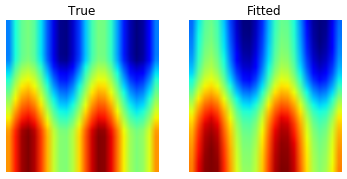
\includegraphics[width=.8\textwidth]{fig_monofair/mixed_monotonicity_demo_1.png}
        \caption{Demonstration of our network architecture's ability to fit a function which is monotonic in one dimension and non-monotonic in another. }
        \label{fig:demo1}
    \end{figure}
        
    To demonstrate the result empirically, we show in Figure~\ref{fig:demo1} a two-dimensional experiment in which the true underlying function is non-monotonic w.r.t to $x_1$ but strictly monotonically increasing w.r.t. $x_2$.  Specifically,
    $$ f(x_1, x_2) = \mbox{sin}(\pi x_1) + \mbox{max}(-1, \mbox{min}(1, x_2))  $$
    
    The estimated function shown is fit on a sample of 1,000 samples from the function and set to be non-monotonic w.r.t. $x_1$ and monotonic w.r.t $x_2$ and is able to recover the true function with reasonable precision.
    
    Similarly, we show in Figure~\ref{fig:demo2} that a mixed-monotonicity function can be fit even if the underlying function is severely non-monotonic (with the expected error in fit).  Here, $f(x_1, x_2) = x_0^2 + x_1^2$, and we again fit on a sample of 1,000 samples from the function and set to be non-monotonic w.r.t. $x_1$ and monotonic w.r.t $x_2$.  As expected, it finds a function which is optimal subject to the (incorrect) constraints.
    
    \begin{figure}
        \centering
        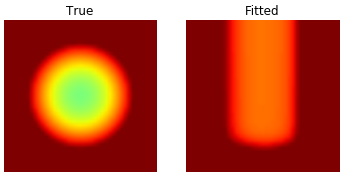
\includegraphics[width=.8\textwidth]{fig_monofair/mixed_monotonicity_demo_2.png}
        \caption{Demonstration of our network architecture's ability to created a function which is monotonic in one dimension and non-monotonic in another, even when the data does not meet those qualifications.}
        \label{fig:demo2}
    \end{figure}


% 
%\appendix 

\chapter{Appendix for Chapter 2}
\label{appendix_B}

\section{Full Conditionals}
\label{sec:full_cond}

We briefly describe the full conditional posterior distributions,
numbered (1) through (9) below, that define the transition
probabilities in the Gibbs sampler MCMC implementation. We define $\bfPsi:=(\bftheta, \bfy)$ as the random vector that includes the full parameter vector as well as the data, and we use the notation $\bfPsi_{-a}$ to represent $\bfPsi$ excluding component $a$.

\begin{enumerate}
\item {\bf Updating $v_{0u},$} $ u = 1, 2, 3$:
  \begin{multline*}
  (v_{0u} \mid \bfPsi_{-v_{0u}}) \sim \mbox{Gamma}\left(a_v + \frac{1}{2}CDL
  \times \kappa_{u}, \right.  \\
  \left. b_v + \frac{1}{2}\sum^C_{c=1} \sum^D_{d=1}
  \sum^L_{\ell=1} \sum^{\kappa_u}_{m=1}(\mu^*_{cd\ell u}(m) -
  \mu_{0u})^2\right).
  \end{multline*}

\item {\bf Updating $\mu_{0u},$} $u = 1, 2, 3$:
  \begin{multline*}
  (\mu_{0u} \mid \bfPsi_{-\mu_{0u}}) \sim N\left(\frac{ v_{0u}\sum^C_{c=1}
  \sum^{D}_{d=1} \sum^L_{\ell=1} \sum^{\kappa_{u}}_{m=1} \mu^*_{cd\ell
    u}(m) + \mu_{00}v_{00} }{ v_{00} + CDL \times \kappa_{u} v_{0u} },
  \right. \\
  \left. \frac{1}{ v_{00} + CDL \times \kappa_{u} v_{0u} }\right).$$
\end{multline*}

\item {\bf Updating $\mu^*_{cd \ell u}$: }
From equation (1), the vector $\bfmu_{cd\ell i}$ can be written as
$$
\bfmu_{cd\ell i} = \mu^*_{cd\ell 1}\left(\delta^1_{cdi}\right)\bfu_1 +
\mu^*_{cd\ell 2}\left(\delta^2_{cdi}\right)\bfu_2 + \mu^*_{cd\ell
  3}\left(\delta^1_{cdi}\right)\bfu_3,
$$
where
$\bfu_1 = (1, \ldots, 1, 0, \ldots, 0)^{\top}$,
$\bfu_2 = (0, \ldots, 0, 1, \ldots, 1, 0, \ldots, 0)^{\top}$
           and
$\bfu_3 = (0, \ldots, 0,\\ 1, \ldots, 1)^{\top}$
with 1's in positions $1,\ldots,\tau^1_{cd\ell}$ (for $\bfu_1$),
in positions $\tau^1_{cd\ell}+1 \ldots \tau^2_{cd\ell}$ (for $\bfu_2$) and
in position $\tau^2_{cd\ell} + 1 \ldots T$ (for $\bfu_3$), respectively.
We find that $(\mu^*_{cd\ell 1}(m) \mid \bfPsi_{-\mu^*_{cd\ell 1}(m)}) \sim N(a_1, b_1)$, with
$b_1 = (v_{01} + J (\#\mathcal{P}^m_{cd1}) \bfu_1^{\top}\bfSigma^{-1}_c
\bfu_1)^{-1}$
and
\begin{multline*}
  a_1 = b_1\, \left[\left(\sum_{i \in \mathcal{P}^m_{cd1}}\sum_j
    \bfy_{cd\ell ij} - J\bfu_2
    \sum_{i \in  \mathcal{P}^m_{cd1}}\mu^*_{cd\ell 2}(\delta^2_{cdi}) -
    J(\#\mathcal{P}^m_{cd1}) \bfu_3 \mu^*_{cd\ell 3}(m) \right)^{\top} \right. \\
    \left.\vphantom{\sum_{i \in  \mathcal{P}^m_{cd1}}} \bfSigma^{-1}_c \bfu_1 + \mu_{01}v_{01} \right],
\end{multline*}
    
  where $\mathcal{P}^m_{cd1} := \{1\leq i \leq I: \delta^1_{cdi} = m \}.$\\
Similarly, $(\mu^*_{cd \ell 2}(m) \mid \bfPsi_{- \mu^*_{cd \ell 2}(m)}) \sim N(a_2, b_2)$, with \\
$  b_2 =(v_{02} + J (\#\mathcal{P}^m_{cd2})
\bfu_2^{\top}\bfSigma^{-1}_c \bfu_2)^{-1}$ and

\begin{multline*}
a_2 = b_2\, \left[\left(
  \sum_{i \in \mathcal{P}^m_{cd2}} \sum_j \bfy_{cd\ell ij} - J\bfu_1
  \sum_{i \in \mathcal{P}^m_{cd2}}\mu^*_{cd\ell 1}(\delta^1_{cdi}) 
  - J\bfu_3
  \sum_{i \in \mathcal{P}^m_{cd\ell 2}}\mu^*_{cd \ell 3}(\delta^1_{cdi})\right)^{\top}\left.\\
     \left. \vphantom{\sum_{i \in \mathcal{P}^m_{cd2}} \sum_j}\bfSigma^{-1}_c \bfu_2 + \mu_{02}v_{02}\right], 
\end{multline*}

where $\mathcal{P}^m_{cd2} := \{1\leq i \leq I: \delta^2_{cdi} = m \}$.\\
And $(\mu^*_{cd \ell 3}(m) \mid \bfPsi_{-\mu^*_{cd \ell 3}(m)}) \sim N(a_3, b_3)$, with \\
$b_3 = (v_{03} + J (\#\mathcal{P}^m_{cd1}) \bfu_3^{\top}\bfSigma^{-1}_c
\bfu_3)^{-1}$ and

\begin{multline*}
  a_3 = b_3\, \left[\left( \sum_{i \in \mathcal{P}^m_{cd1}} \sum_j \bfy_{cd\ell ij} - J\bfu_2 \sum_{i \in \mathcal{P}^m_{cd1}}\mu^*_{cd\ell 2}(\delta^2_{cdi}) - J(\#\mathcal{P}^m_{cd1})\bfu_1 \mu^*_{cd\ell 1}(m) \right)^{\top} \right.\\
\left. \vphantom{\sum_{i \in \mathcal{P}^m_{cd2}} \sum_j}    \bfSigma^{-1}_c\bfu_3 + \mu_{03}v_{03}\right].
\end{multline*}
%
\item {\bf Updating $\bfSigma_c$: }
Under the normal-inverse Wishart conjugate model we get
\begin{multline*}
(\bfSigma_c \mid \bfPsi_{-\bfSigma_c}) \sim IW\left( IDLJ + \nu_{\Sigma}, \vphantom{\sum^J_{j=1}}\right. \\
\left. \sum^I_{i=1} \sum^D_{d=1} \sum^L_{\ell=1}
\sum^J_{j=1}(\bfy_{cdi\ell j} - \bfmu_{cd\ell i} )(\bfy_{cdi\ell j} -
\bfmu_{cd\ell i} )^{\top} + V_{\Sigma_c} \right)
\end{multline*}
%
\item {\bf Updating $\gamma$: }
\begin{multline*}
  (\gamma \mid \bfPsi_{-\gamma}) \sim \mbox{Beta}\left( a_{\gamma} + \sum^C_{c=1}
  \sum^D_{d=1} \sum^I_{i=1} \mathds{1}(\delta^2_{cdi} = \delta^1_{cdi}),
 \right. \\ 
  \left. b_{\gamma} + 
  \sum^C_{c=1} \sum^D_{d=1} \sum^I_{i=1} \mathds{1}(\delta^2_{cdi} \neq
  \delta^1_{cdi} ) \right)
\end{multline*}
%
\item {\bf Updating $\tau^1_{cd\ell}$ and $\tau^2_{cd\ell}$: }
We update $\tau^1_{cd\ell}$ and $\tau^2_{cd\ell}$ in different blocks of
the Gibbs sampler. This way we evaluate fewer scenarios than in the
case of sampling both together in a single step, due to the
restriction $\tau^1_{cd\ell}<\tau^2_{cd\ell}$.
\begin{gather}
 p(\tau^1_{cd\ell} \mid \bfPsi_{-\tau^1_{cd\ell}} ) \propto \prod^I_{i=1}
 \prod^J_{j=1} N(\bfy_{cd\ell ij}; \bfmu_{cd\ell i}, \bfSigma_c), \ \ \
 \tau^1_{cd\ell}<\tau^2_{cd\ell}. \nonumber \\
 p(\tau^2_{cd\ell} \mid \bfPsi_{-\tau^2_{cd\ell}} ) \propto \prod^I_{i=1}
 \prod^J_{j=1} N(\bfy_{cd\ell ij}; \bfmu_{cd\ell i}, \bfSigma_c), \ \ \
 \tau^1_{cd\ell}<\tau^2_{cd\ell}.
 \label{eq:tau}
\end{gather}
If evaluating the probabilities in \eqref{eq:tau} is too
computationaly intensive, one can alternatively implement
a Metropolis-Hastings transition probability, proposing 
% for sampling from each conditional proposing
unit increments or decrements, subject to the constraint
$\tau^1_{cd\ell}<\tau^2_{cd\ell}$. This would require at most
four evaluations of the right hand side product in \eqref{eq:tau}.  \ech

\item {\bf Updating cluster membership indicators $\delta^1_{cdi}$: }
  If $\delta^2_{cdi}\leq \kappa_1$, then $\delta^1_{cdi}$ is equal to the value of
  $\delta^2_{cdi}$ with probability 1. Otherwise, by multinomial-Dirichlet
  conjugacy results, the full conditional distribution of
  $\delta^1_{cdi}$ is
  $
  P(\delta^1_{cdi} =m \mid \bfPsi_{-\delta^1_{cdi}}) \propto
  \NN^1_{cdi}(m)\pi^1_{m}$, 
  $m=1,\ldots,\kappa_1$ 
%         \sim \mbox{Multinomial}\left((1, \ldots, \kappa_1); \ \ \
% (, \ldots,
%   \NN^1_{cdi}(\kappa_1)\pi_{1
%     \kappa_1})/\sum^{\kappa_1}_{m=1}\NN^1_{cdi}(m)\pi_{1m}\right),
%   $$
where $\NN^1_{cdi}(m)=\prod_{\ell} \prod_j N(\bfy_{cd\ell ij} \mid
\bfmu_{cd\ell i}, \bfSigma_c )$ with $\bfmu_{cd\ell i}$ evaluated under
$\delta^1_{cdi}=m$. 
%
\item {\bf Updating cluster membership indicators $\delta^2_{cdi}$: }
The full conditional p.m.f. for $\delta^2_{cdi}$ is given by
\begin{equation*}
P(\delta^2_{cdi} = m \mid \bfPsi_{-\delta^2_{cdi}}) \propto
\begin{cases}
  \gamma \times \NN^2_{cdi}(\delta^1_{cdi} )
  %{ \gamma  \NN^2_{cdi}(\delta^1_i ) + (1-\gamma) \sum^{\kappa_2 -
  %\kappa_1}_{m=\kappa_1+1} \pi^2_{m-\kappa_1}\NN^2_{cdi}(m) }, \ \ \
  & \mbox{ if } m =  \delta^1_{cdi}.\\ 
  (1-\gamma) \times \pi^2_{m-\kappa_1}  \NN^2_{cdi}(m)
  % { \gamma \NN^2_{cdi}(\delta^1_i) + (1-\gamma) \sum^{\kappa_2 -
  %   \kappa_1}_{m=\kappa_1+1} \pi_{2, m-\kappa_1}\NN^2_{cdi}(m)},   \ \ \ 
  & \mbox{ if } \kappa_1+1\leq m \leq \kappa_2.
\end{cases}
\end{equation*}
where $\NN^2_{cdi}(m)=\prod_{\ell} \prod_j
N(\bfy_{cd\ell ij} \mid \bfmu_{cd\ell i}, \bfSigma_c )$ with $\bfmu_{cd\ell
i}$ being calculated assuming $\delta^2_{cdi}=m$. 
%
\item {\bf Updating $\bfpi_{1}$ and $\bfpi_2$: }
under the conjugate multinomial-Dirichlet model we
find the following posterior distribution.
Let 
$n^1_m = \sum^C_{c=1} \sum^D_{d=1} \\ \sum^I_{i=1}
\mathds{1}(\delta^1_{cdi}=m)$. 
for $m=1, \ldots, \kappa_1$.
Similarly, let 
$n^2_m = \sum^C_{c=1} \sum^D_{d=1}$ $\sum^I_{i=1} \mathds{1}(\delta^2_{cdi}=m)$ for 
$m=\kappa_1+1,\ldots,\kappa_1+\kappa_2$.
Then $
  (\bfpi_1 \mid \bfPsi_{-\bfpi_1}) \sim \Dir(\eta_{11}     +n^1_1,\ldots,
                               \eta_{1\kappa_1}+n^1_{\kappa_1})
$
and
%   \mbox{Dirichlet}\left( \eta_{11} +
% , \ \ldots\  \right. \\
%   &\hspace{5 cm} \left. \ \ldots \ , \ \eta_{1 \kappa_1} + \sum^C_{c=1} \sum^D_{d=1} \sum^I_{i=1} \mathds{1}(\delta^1_{cdi}=\kappa_1) \right).
$
(\bfpi_2 \mid \bfPsi_{-\bfpi_2}) \sim \Dir(\eta_{21}+n^2_{\kappa_1+1}, \ldots, 
                     \eta^2_{\kappa_2-\kappa_1} +n^2_{\kappa_1+\kappa_2}). 
$

% \begin{align*}
%   (\bfpi_2 \mid \ldots) &\sim \mbox{Dirichlet}\left( \eta_{21} + \sum^C_{c=1} \sum^D_{d=1} \sum^I_{i=1} \mathds{1}(\delta^2_{cdi}=1 + \kappa_1),  \ \ldots \ \right. \\
%   &\hspace{5 cm} \left. \ \ldots \ , \ \eta_{2, \kappa_2 - \kappa_1} + \sum^C_{c=1} \sum^D_{d=1} \sum^I_{i=1} \mathds{1}(\delta^2_{cdi}=\kappa_2) \right) .
% \end{align*}
\end{enumerate}


\section{Number of Model Parameters for AIC and BIC}
\label{sec:number_param}

Here we describe how the number of parameters was determined when
evaluating the BIC criterion in sections 4 and 5 and
AIC in section 4. The description focuses on BIC, but
the same arguments are valid for evaluation of AIC. 

The number of parameters for a given model is a function of $\kappa_1$ and
$\kappa_2$ that can be decomposed as $N(\kappa_1, \kappa_2) = f( \kappa_1,
\kappa_2) + const$, where $const$ depends on the number of data points,
but not on $\kappa_1$ or $\kappa_2$. 
The only parameters in the likelihood that vary in number as $\kappa_1$ and
$\kappa_2$ change are
$\{\bfmu^*_{\ell ,u}: c\in [C], d\in [D], \ell \in [L], u \in [3] \}$,
which contains
$f(\kappa_1, \kappa_2) = CDL(2\kappa_1 + \kappa_2)$ parameters.
Therefore, $BIC = 2 \log p(\bfy \mid \theta) 
- N(\kappa_1, \kappa_2) \log n,$ where $n$ is the number of observations,
hence the comparison of any pair of models is invariant with respect to
the term $const$ and we can, for simplicity, consider $N(\kappa_1,
\kappa_2) = CDL(2\kappa_1 + \kappa_2)$.


% 
%\appendix 

\chapter{Appendix for Chapter 3}
\label{appendix_C}

\section{Proper Prior on $(\bfmu_1, \ldots, \bfmu_k, b_1, \ldots, b_k, k)$}
\label{sec:proper_prior}

Here we show that $p(\bfmu_1, \dots, \bfmu_k, \bfb, k)$ defined in \eqref{eq:prior1} is a proper prior. In fact, since 

$$ \exp\left\{- \alpha \sum_{j=1}^k d(\bfmu_j, \bfmu_{b_j}) \right\}<1, \ \ \ \ \forall \ 1 \leq j \leq k,$$

\noindent it follows that

$$Z_k \leq \int \dots \int_{\mathbb{R}^{p \times k}} \prod_{j=1}^k \left[ p(\bm{\mu}_j)\right]k^k \ d\bfmu_1 \dots  d\bfmu_k = k^k < \infty.$$

\noindent Without loss of generality, we can truncate $P(k)$ to have suport $1\leq k \leq M$ for some finite upper limit $M$ and therefore $p(k)$ will be also proper. The truncation is justified in practical appications since one expects finite number of nodes in the tree.


\section{Full Conditional Distributions for the s-MST Model}
\label{sec:app_smst}

We now describe posterior inference under the s-MST model of Section \ref{sec:soft_mst}. A simple MCMC can be implemented in such a scenario, leading to the Gibbs sampling transition probabilities:
\begin{enumerate}
\item Updating $c_i$:
\begin{align*}
p (c_i = k | \bm{y}_i, \bfmu_k, \Sigma, w_k) &\propto L(\bm{y}_i | c_i = k, \bfmu_k, \Sigma) \ p(c_i = k | w_k)
\\
&\propto w_k \ \mathcal{N} (\bm{y}_i; \bfmu_{k}, \Sigma), \quad \forall k = 0, \dots, k.
\end{align*}

\item Updating $\bm{w}$:
\begin{align*}
p(\bm{w} | c_1, \dots, c_n) &\propto p(c_1, \dots, c_n | \bm{w}) \ p(\bm{w})
\\
&\sim \mbox{Dirichlet} (n_0 + \delta, \dots, n_k + \delta).
\end{align*}

%\item Updating $\Sigma_k, \forall k = 0, \dots, K$:
%\begin{align*}
%p (\Sigma_k | Y ,  \mbox{rest}) &\propto L(Y | c_1, \dots, c_n,  \bfmu_k, \Sigma_k) \ p(\Sigma_k)
%\\
%&\propto \prod_{i : c_i = k} \left\{ |\Sigma_k|^{-\frac{1}{2}} e^{-\frac{1}{2} (\bm{x}_i - \bfmu_k)^T \Sigma_k^{-1} (\bm{x}_i - \bfmu_k)} \right\} |\Sigma_k|^{- \frac{\nu + p + 1}{2}} e^{ - \frac{1}{2} \mbox{tr} (R \Sigma_k^{-1})}
%\\
%&\sim \mathcal{IW} \left( \nu + n_k, \Psi + \sum_{i : c_i = k} (\bm{y}_i - \bfmu_k)(\bm{y}_i - \bfmu_k)^T \right).
%\end{align*}
%In the case of unique covariance matrix $\Sigma$, we use all data points to update the parameters, obtaining $p (\Sigma | Y ,  \mbox{rest}) \sim \mathcal{IW} \left( \nu + n, \Psi + \sum_{i} (\bm{y}_i - \bfmu_k)(\bm{y}_i - \bfmu_k)^T \right)$.

\item Updating $\Sigma$:
\begin{align*}
p (\Sigma | Y ,  \mbox{rest}) &\propto L(Y |  \bfmu_k, c_1, \dots, c_n, \Sigma) \ p(\Sigma)
\\
&\propto \prod_{i=1}^n \left\{ |\Sigma|^{-\frac{1}{2}} e^{-\frac{1}{2} (\bm{x}_i - \bfmu_{c_i})^T \Sigma^{-1} (\bm{x}_i - \bfmu_{c_i})} \right\} |\Sigma|^{- \frac{\nu + p + 1}{2}} e^{ - \frac{1}{2} \mbox{tr} (R \Sigma^{-1})}
\\
&\sim \text{Inv-Wishart} \left( \nu + n, \Psi + \sum_{i} (\bm{y}_i - \bfmu_{c_i})(\bm{y}_i - \bfmu_{c_i})^T \right).
\end{align*}


\item Updating $\bfmu_k, \forall k = 1, \dots, k$:
\begin{align*}
p (\bfmu_k | Y, \mbox{rest}) &\propto L(Y | c_1, \dots, c_n,  \bfmu_k, \Sigma) \ p(\bfmu_j | \bfmu^{(-j)}, \bfb, \alpha, k)
\\
&\sim \mathcal{N} \left((\Sigma_p^{-1} + n_j \Sigma^{-1})^{-1} \left[\Sigma_p^{-1} \bfmu_p + \Sigma^{-1} \sum_{i:c_i = j} \bfy_i \right] , \\
&\left. \hspace{6 cm}(\Sigma_p^{-1} + n_j \Sigma^{-1})^{-1} \vphantom{ \sum_{i:c_i = j}} \right),
\end{align*}
where $f_j, \bfmu_p, \Sigma_p$ were defined in equations \eqref{eq:mu_cond_eucl1} and \eqref{eq:mu_cond_eucl2}.


\item Updating the branching structure: by resampling it from the prior conditionals $p(b_j = i | \bfmu_0, \dots, \bfmu_k, \bfb^{(-j)},  k)$ described in \eqref{eq:b_cond}.

%\item Updating the hyperparameter $\alpha$. We can use a Gamma prior (or Exponential), getting posterior conjugacy, i.e. 
%$$p(\alpha | \bfmu_0, \dots, \bfmu_K, \bfb, K) \sim \text{Gamma} \left(a_\alpha, b_\alpha + \sum_{j=1}^K d(\bfmu_j, \bfmu_{b_j}) \right)$$
%\textbf{This full conditional is still problematic because values of $\alpha$ too small are sampled. This, in turn, implies the sampling of trees that are not repulsive MST.}

\item Updating the dimension $K$ using a RJ-MCMC move:
\begin{enumerate}
\item Generate a proposal $\tilde{k} \sim q(\tilde{k} | k)$ and a matching set of parameters $\tilde{\bm{\theta}}_{\tilde{k}} \sim p_1(\tilde{\bm{\theta}}_{\tilde{k}} | y^\prime)$ as described in Section \ref{sec:mst_inference}
}
\item Accept $(\tilde{k}, \tilde{\bm{\theta}}_{\tilde{k}})$ with probability $\alpha$ defined in \eqref{eq:alpha}.
\end{enumerate}
\end{enumerate}

\section{Full Conditional Distributions for the h-MST Model}
\label{sec:app_hmst}

First, we list the full conditional distributions for implementation of Gibbs sampler on the model described in Section \ref{sec:model2_mst} conditionaly on the dimension $k$.

\begin{enumerate}

\item Updating $c_j$:

\begin{align*}
p (c_i = j | \bm{y}_i, \bfmu_j, \Sigma_j, w_j, k) &\propto L(\bm{y}_i | c_i = j, \bfmu_j, \Sigma) \ p(c_i = j | w_j)
\\
&\propto w_j \ \mathcal{N} (\bm{y}_i; \bfmu_{j}, \Sigma_j), \quad \forall j = 0, \dots, k.
\end{align*}

\item Updating $\bm{w}$:
\begin{align*}
p(\bm{w} | c_1, \dots, c_n, k) &\propto p(c_1, \dots, c_n | \bm{w}, k) \ p(\bm{w} \mid k)
\\
&\sim \mbox{Dirichlet} (n_0 + \delta, \dots, n_k + \delta).
\end{align*}

%\item Updating $\lambda_{jd}$:
%\begin{align*}
%p(\lambda_{jd} \mid \bfy, \bfmu, \Sigma, \bfc, k) &\propto \prod_{i \in S_j}%p(\bfy_i \mid \bfmu_j, \Sigma_j, c_i, k) p(\lambda_jd)\\
%& \sim \mbox{InvGamma}\left( \frac{\#S_j}{2} + a, \ \frac{1}{2} \sum_{i \in S_j}(y_i - \bfmu_j)^T\bfe_d\bfe_d^{\top}(y_i - \bfmu_j) + b\right),
%\end{align*}

%\noindent where $S_j := \{i: \ c_i=j\}$ and $\bfe_d$ denotes the $d$-th eigenvalue of $\Sigma_j$ (which is also the $d$-th column of $\bfE$).

\item Updating $\Sigma^{-1}$

\begin{align*}
p(\Sigma^{-1} \mid \bfy, rest) &\propto \prod^n_{i=1} p(\bfy_i \mid \bfmu_{c_i}, \Sigma^{-1})p(\Sigma^{-1})\\
&\sim Wishart \left( n + \nu, \left[ \Psi^{-1} + \sum^{n}_{i}(\bfy_i - \bfmu_{c_i})(\bfy_i - \bfmu_{c_i})^{\top} \right]^{-1}\right).
\end{align*}

\item Updating $\bfmu_j$:

The conditional posterior density $p(\bfmu_j\mid \bfy, \mbox{rest})$ is not straightforward to either write in analytic form or to sample from. 

Denote by $S_j:=\{i: \ c_i=j\}$ the set of observations that belong to cluster $j$. Combining the likelihood with the h-MST prior, we have

\begin{align*}
p(\bfmu_j \mid \bfmu^{(-j)}, \bfy, rest)&\propto \left[\prod_{i\in S_j} N(\bfy_i; \bfmu_{j}, \Sigma) N(\bfmu_j; \bfm, \sigma^2_0I)\right]\times \\
& \hspace{3 cm}\times\exp\left\{-\alpha\mathcal{W}( MST(\bfmu_1, \cdots, \bfmu_k) ) \right\},
\end{align*}

\noindent in which the sum $\mathcal{W}( MST(\bfmu_1, \cdots, \bfmu_k) )$ involves different terms depending on the position of $\bfmu_j$ in $\mathbb{R}^D$. This leads to the full conditional being a finite mixture of truncated normals, with non-overlapping truncation regions $A_l\subset \mathbb{R}^D, \ l=1, \ldots, n$ such that the neighbors of any node $\bfmu_j\in A_l$ are the same under the $MST(\bfmu_1, \ldots, \bfmu_k)$ when we fix the remaining nodes $\bfmu^{(-j)}$. The challenge lies in defining the regions $A_l$ that partition $\mathbb{R}^D$.

However, we can build a tractable and efficient Metropolis Hastings proposal $q(\tilde{\bfmu}_j \mid \bfmu_j; \bfmu^{(-j)}, \bfy, rest)$ to approximate $p(\bfmu_j\mid \bfy, \mbox{rest})$. We will omit the dependence on variables other than $\bfmu_j$ from the notation for clarity of exposition, therefore writing $q(\tilde{\bfmu}_j \mid \bfmu_j)$ instead of $q(\tilde{\bfmu}_j \mid \bfmu_j; \bfmu^{(-j)}, \bfy, rest)$. We define $q(\tilde{\bfmu}_j \mid \bfmu_j)$ as follows. Take from the edges $E_{\bfmu_1, \ldots, \bfmu_k}$ of the $MST(\bfmu_1, \ldots, \bfmu_k)$  the subset $V_j=\{i: \ \{j,i\} \in E_{\bfmu_1, \ldots, \bfmu_k} \}$ of all neighbors of node $j$. We propose a new component specific mean $\tilde{\bfmu}_j$ from


\begin{align*}
q(\tilde{\bfmu}_j \mid \bfmu_j)\propto \prod_{i\in S_j} N(\bfy_i; \tilde{\bfmu}_{j}, \Sigma) N(\tilde{\bfmu}_j; \bfm, \sigma^2_0I) \exp\left\{-\alpha\sum_{i \in V_j} d^2(\bfmu_i, \tilde{\bfmu}_j) \right\},
\end{align*}

\noindent which simplifies to $q(\tilde{\bfmu}_j \mid \bfmu_j)\sim N(\tilde{\bfmu_j}; \ \bfa_j, \bfB_j),$ where \ $\bfB_j = ( |S_j| \Sigma^{-1} +$ $\sigma^{-2}_0 I + 2\alpha |V_j|I )^{-1}$ and \ $\bfa_j = \bfB_j\left( \Sigma^{-1} \sum_{i \in S_j}\bfy_i + \sigma^{-2}_0\bfm + 2\alpha\sum_{l \in V_j}\bfmu_l\right).$ By denoting the proposed neighborhood of $\tilde{\bfmu}_j$ as $\tilde{V}_j=\{i: \{i,j\} \in E_{\bfmu^*_1, \ldots, \bfmu^*_k}\}$ where $\bfmu^*_l = \bfmu_l$ if $l\neq j$ and $\bfmu^*_j = \tilde{\bfmu}_j$, the resulting Metropolis Hastings acceptance probability equals 1 if $\tilde{V}_j = V_j$ and

\begin{align*}
\alpha&( \tilde{\bfmu}_j \mid \bfmu_j) = \min\left\{ 1, \frac{q(\bfmu_j \mid \tilde{\bfmu_j}) p(\tilde{\bfmu}_j\mid \bfy)}{q(\tilde{\bfmu}_j \mid \bfmu_j)p(\bfmu_j \mid \bfy))}\right\}\\
&=\min \left\{ 1, \ \ \frac{ \left[ \prod_{i\in S_j} N(\bfy_i; \tilde{\bfmu}_j, \Sigma_{j}) \right] N(\tilde{\bfmu}_j; \bfm, \sigma^2_0I)}{   \left[ \prod_{i\in S_j} N(\bfy_i; \bfmu_j, \Sigma_j) \right] N(\bfmu_j; \bfm, \sigma^2_0I) } \times \right.\\
&\hspace{2 cm} \times \left. \frac{\exp\left\{-\alpha\mathcal{W}( MST(\tilde{\bfmu}_j, \bfmu^{(-j)}) ) \right\}}{\exp\left\{-\alpha\mathcal{W}( MST(\bfmu_1, \cdots, \bfmu_k) ) \right\} } \times \frac{N(\bfmu_j; \ \tilde{\bfa}_j, \tilde{\bfB}_j)}{N(\tilde{\bfmu}_j; \ \bfa_j, \bfB_j)} \right\}
\end{align*}
\begin{align*}
\ \ \ \ =\min \left\{1, \ \ \frac{ \left[ \prod_{i\in S_j} N(\bfy_i; \tilde{\bfmu}_j, \Sigma_{j}) \right] N(\tilde{\bfmu}_j; \bfm, \sigma^2_0I) }{   \left[ \prod_{i\in S_j} N(\bfy_i; \bfmu_j, \Sigma_j) \right] N(\bfmu_j; \bfm, \sigma^2_0I)}\frac{N(\bfmu_j; \ \tilde{\bfa}_j, \tilde{\bfB}_j)}{N(\tilde{\bfmu}_j; \ \bfa_j, \bfB_j)} \right. \times\\
\times\left. \frac{\exp\left\{-\alpha \sum_{i \in \tilde{V}_j} d^2(\tilde{\bfmu}_j, \bfmu_i) \right\}}{  \exp\left\{-\alpha\sum_{i \in V_j} d^2(\bfmu_j, \bfmu_i) \right\}  } \right\}
\end{align*}

\noindent otherwise.

\end{enumerate}

% 
%\appendix 

\chapter{Appendix for Chapter 4}
\label{appendix_D}

\section{Full Conditionals for the POE Model}
\label{sec:full_cond}
\vspace{0.3 cm}

Here we briefly describe how to sample from each one of the full conditionals. In this section, we use $\mathds{1}(\cdot)$ to denote either an indicator function or th support of a truncated probability distribution. We also define the sets $\mathcal{P}^+_g:=\{ 1\leq t \leq T: \ e_{sg} = 1\}$ and $\mathcal{P}^+_t:=\{ 1\leq g \leq G: \ e_{sg} = 1\}$. The sets $\mathcal{P}^0_g, \ \mathcal{P}^-_g, \ \mathcal{P}^0_t$ and $\mathcal{P}^-_t$ are defined analogously.\\

\textbf{Updating $e_{sg}$}

$$p(e_{sg} = x \mid y, else) \propto \begin{cases}
\frac{\pi^+_g}{k^+_g} \times \mathds{1}(\alpha_s + \mu_g < y_{sg} < \alpha_s + \mu_g + k^+_g), &\mbox{ if } x = 1,\\
\pi^0_g \times N(y_{sg}; \ \alpha_s + \mu_g, \ \sigma^2_g), &\mbox{ if } x = 0,\\
\frac{\pi^-_g}{k^-_g} \times \mathds{1}(\alpha_s + \mu_g - k^-_g < y_{sg} < \alpha_s + \mu_g), &\mbox{ if } x = -1.
\end{cases}$$\\

\textbf{Updating $k^+_g$ and $k^-_g$}

\begin{multline*}
(k^+_g \mid y, else) \sim InvGamma(\# \mathcal{P}^+_g + \alpha_{k^+}, \ \beta_{k^+})\\
\mathds{1}\left(k^+_g > \max \left(\max_{t \in \mathcal{P}^+_g}\{y_{sg} - \alpha_s -\mu_g\}, \ k_0 \sigma_g \right) \right).
\end{multline*}

\begin{multline*}
(k^-_g \mid y, else) \sim InvGamma(\#\mathcal{P}^-_g + \alpha_{k^-}, \ \beta_{k^-})\\
\mathds{1}\left(k^-_g > \max \left(\max_{t \in \mathcal{P}^-_g }\{\alpha_s +\mu_g - y_{sg}\}, \ k_0 \sigma_g \right) \right).
\end{multline*}

\textbf{Updating $\bfpi_{g}$}

$$(\bfpi_g \mid y, else) \sim Dirichlet \left( (\ \#\mathcal{P}^-_g + \alpha^-_{\pi}, \ \#\mathcal{P}^0_g + \alpha^0_{\pi}, \ \#\mathcal{P}^+_g + \alpha^+_{\pi}) \right).$$

\textbf{Updating $\sigma^2_{g}$}

\begin{multline*}
(\sigma^2_g \mid y, else) \sim InvGamma \left( \frac{\#\mathcal{P}^0_g }{2} + \gamma, \ \frac{1}{2} \sum_{t \in \mathcal{P}^0_g } (y_{sg} - \alpha_s - \mu_g)^2 + \lambda\right)\\
\mathds{1}\left( \sigma^2_g < \frac{\min \left( k^+_g, k^-_g\right)^2}{k^2_0} \right).
\end{multline*}

\textbf{Updating $\mu_g$}

$$(\mu_g \mid y, else) \sim N(a_g, b_g) \mathds{1}\left( \max\left(M^+_g, M^-_g\right) < \mu_g < \min\left(m^{+}_g, m^-_g \right)\right),$$ 

where 
\begin{align*}
M^+_g &= \max\{y_{sg} - \alpha_s; \ t \in \mathcal{P}^+_g\} - k^+_g; \\ 
M^-_g &= \max\{y_{sg} - \alpha_s; \ t \in \mathcal{P}^-_g\}; \\ 
m^+_g &= \min\{y_{sg} - \alpha_s; \ t \in \mathcal{P}^+_g\}; \\ 
m^+_g &= \min\{y_{sg} - \alpha_s; \ t \in \mathcal{P}^-_g\} + k^-_g;\\
b_g &= (\#\mathcal{P}^0_g \sigma^{-2}_g + \tau^{-1}_{\mu})^ {-1};\\
a_g &= b_g \times \left[ \sigma^{-2}_g \sum_{t \in \mathcal{P}^0_g}(y_{sg} -\alpha_s ) + \tau^{-1}_{\mu}\theta_{\mu}\right]. 
\end{align*}

\textbf{Updating $\alpha_s$}
\begin{multline*}
(\alpha_s \mid y, else) \sim N( a_t, b_t) \\
\mathds{1}\left( \max\left(M^+_t, M^-_t\right) < \alpha_s < \min\left(m^{+}_t, m^-_t \right)\right)\mathds{1}\left(\sum^T_{t=1} \alpha_s = 0\right).
\end{multline*}

where
\begin{align*}
M^+_t &= \max\{y_{sg} - \mu_g - k^+_g; \ g \in \mathcal{P}^+_t\}; \\ 
M^-_t &= \max\{y_{sg} - \mu_g; \ g \in \mathcal{P}^-_t\}; \\ 
m^+_t &= \min\{y_{sg} - \mu_g; \ g \in \mathcal{P}^+_t\}; \\ 
m^+_t &= \min\{y_{sg} - \mu_g + k^-_g; \ g \in \mathcal{P}^-_t\};\\
b_t &= \left( \sum_{ g \in \mathcal{P}^0_t} \sigma^{-2}_g + \tau^{-1}_{\alpha} \right)^ {-1};\\
a_t &= b_t \times \left[ \sum_{t \in \mathcal{P}^0_t} \left( \frac{y_{sg} -\alpha_s}{\sigma^{2}_g } \right) + \tau^{-1}_{\alpha} \mu_{\alpha}\right]. 
\end{align*}

\textbf{Updating $\theta_{\mu}$}

$$(\theta_{\mu} \mid y, else) \sim N \left( \left(m_{\mu}s^{-2}_{\mu} + \tau^{-1}_{\mu}\sum^G_{g=1} \mu_g\right)(s^{-2}_{\mu} + G\tau^{-1}_{\mu})^{-1}, \ (s^{-2}_{\mu} + G\tau^{-1}_{\mu})^{-1}\right)$$

\textbf{Updating $\tau_{\mu}$}

$$(\tau_{\mu} \mid y, else) \sim InvGamma \left( \frac{G}{2} + a_{\tau_{\mu}}, \ \frac{1}{2} \sum^G_{g=1}(\mu_g - \theta_{\mu})^2 + b_{\tau_{\mu}}\right)$$

\textbf{Updating $\beta_{k^+}$}

$$ (\beta_{k^+} \mid y, else) \sim Gamma\left(G \alpha_{k^+} + a_{\beta_{k^+}}, \ b_{\beta_{k^+}} + \sum^G_{g=1}\frac{1}{k^+_g}\right)$$

\textbf{Updating $\beta_{k^-}$}

$$ (\beta_{k^-} \mid y, else) \sim Gamma\left(G \alpha_{k^-} + a_{\beta_{k^-}}, \ b_{\beta_{k^-}} + \sum^G_{g=1}\frac{1}{k^-_g}\right)$$

\textbf{Updating $\alpha_{k^+}$}

$p(\alpha_{k^+} \mid y, else)$ is not analytically available since

$$p(\alpha_{k^+} \mid y, else) \propto \Gamma(\alpha_{k^+})^{-G} \left( \frac{\beta^G_{k^+}}{ \prod^G_{g=1}k^+_g}\right)^{\alpha_{k^+}}e^{-\alpha_{k^+}\lambda_{\alpha_{k^+}}}.$$

One way of (approximately) sampling from this distribution is through the Metropolis-Hastings scheme. 

We specify a proposal $q(\alpha^{new}_{k^+} \mid \alpha^{old}_{k^+})$ corrected by the acceptance probability $\alpha(\alpha^{new}_{k^+} \mid \alpha^{old}_{k^+}):=\min\left\{1, \  r(\alpha^{new}_{k^+} \mid \alpha^{old}_{k^+}) \right\},$ where

$$r(\alpha^{new}_{k^+} \mid \alpha^{old}_{k^+}) := \frac{q(\alpha^{old}_{k^+} \mid \alpha^{new}_{k^+})p(\alpha^{new}_{k^+} \mid y, else)}{q(\alpha^{new}_{k^+} \mid \alpha^{old}_{k^+})p(\alpha^{old}_{k^+} \mid y, else)}.$$

Our proposal is a random-walk on $\log \alpha_{k^+},$ i.e., $\log \alpha^{new}_{k^+} \sim N(\log\alpha^{old}_{k^+}, V^+)$ for some fixed $V^+>0$. which implies a LogNormal proposal density on the original scale with $q(\alpha^{new}_{k^+} \mid \alpha^{old}_{k^+}) = N(\alpha^{new}_{k^+}; \alpha^{old}_{k^+}, V^+)\times 1/\alpha^{new}_{k^+}$.

It is straightforward to verify that
\begin{align*}
\log r(\alpha^{new}_{k^+} \mid \alpha^{old}_{k^+}) = (\log \alpha^{old}_{k^+} &- \log \alpha^{new}_{k^+}) - G\left[ \log \Gamma(\alpha^{new}_{k^+}) - \log \Gamma(\alpha^{old}_{k^+}) \right] + \\
&+(\alpha^{new}_{k^+} - \alpha^{old}_{k^+}) \left[  G \log \beta_{k^+} - \sum^G_{g=1} \log k^+_g - \lambda_{\alpha_{k^+}}\right].
\end{align*}

\textbf{Updating $\alpha_{k^-}$}

Updating $\alpha_{k^-}$ is entirely analogous to updating $\alpha_{k^+}$.

\subsection{Sampling from truncated distributions within MCMC}
\label{sec:trunc_dists}

In this section we describe the Gibbs sampler augmentation scheme to asymptotically sample from the truncated inverse gamma and truncated normal distributions that appear in appendix \ref{sec:full_cond}. Although sampling algorithms for truncated distributions can be easy derived, sometimes even by the inverse c.d.f. method, the resulting algorithm can often be numerically unstable (take the truncated Gaussian distribution for example). In such cases, it could be advantageous to use an approximate sampler if it is more robust to computational errors. In this regard, we follow the directions on \cite{damien2001}. 

The univariate normal sampling scheme can be seen as a particular instance of the algorithm for multivariate normals or as an extension of the sampling scheme for univariate standard normals that are both described in \cite{damien2001}. The algorithm to sample from truncated inverse gamma is very similar to the one that samples from the truncated Gamma. We describe both sampling schemes here solely for the purpose of completeness.


\subsubsection{Truncated normal}

Suppose a truncated Gaussian distribution for the random variable $X$: $X\sim N(\mu, \sigma^2)\mathds{1}(a < X < b)$, i.e., $f_{X}(x) \propto \exp\left\{-\frac{(x - \mu)^2}{2 \sigma^2} \right\}\mathds{1}(a < x<b)$, where we could have $a=-\infty$ or $b=+\infty$ to represent unilateral truncation. We define the auxiliary variable $Y$ through the joint density

$$f_{X,Y}(x, y) \propto \mathds{1}(0<y<e^{-\frac{(x-\mu)^2}{2\sigma^2}})\mathds{1}(a<x<b)$$

\noindent so that the implied marginal for $X$ matches the original $N(\mu, \sigma^2)\mathds{1}(a < X < b)$. The full conditional distributions are 

\begin{align}
(Y\mid X=x) &\sim Unif\left(0, \ \exp\left\{-\frac{(x - \mu)^2}{2\sigma^2}\right\}\right),\label{eq:trunc_normal_1}\\
(X \mid Y=y) &\sim Unif\left(\max (a, \ \mu - \sqrt{-2\sigma^2\log y}), \ \ \min (b, \ \mu + \sqrt{-2\sigma^2\log y})\right).\label{eq:trunc_normal_2}
\end{align}

Within the MCMC scheme described in section \ref{sec:full_cond}, we include sampling from the auxiliary variables $Y_{\mu_g}$ and $Y_{\alpha_t}$ corresponding to the full conditional distributions of $\mu_g$, and $\alpha_t$ respectively. The auxiliary variables are sampled from \eqref{eq:trunc_normal_1} while the original variables are sampled from \eqref{eq:trunc_normal_2}, with the appropriate values of $\mu$, $\sigma^2$, $a$ and $b$.


\subsubsection{Truncated inverse gamma}

Suppose $X \sim InvGamma(\alpha, \beta)\mathds{1}(a<x<b)$, i.e., $f_{X}(x) \propto x^{-\alpha -1} e^{-\frac{x}{\beta}}\\ \mathds{1}(a < x < b).$ We define the joint density of $X$ and $Y$:

$$f_{X,Y}(x, y) \propto x^{-\alpha - 1} \mathds{1}(0<y<e^{-\frac{x}{\beta}})\mathds{1}(a<x<b)$$

\noindent so that the implied marginal for $X$ matches the original $InvGamma(\alpha, \beta)\mathds{1}(a<X<b)$. The full conditional distributions are 
\begin{align}
(Y \mid X=x) \sim Unif(0, e^{-\frac{x}{\beta}}),\label{eq:trunc_gamma_inv1} \\
f_{X\mid Y}(x \mid y) \propto x^{-\alpha -1} \mathds{1}(M(y)<x<b),
\label{eq:trunc_gamma_inv2}
\end{align}

\noindent where $M(y):=\max\left( a, \ -\frac{\beta}{\log y}\right)$. The inverse c.d.f. method provides an efficient way to sample from \eqref{eq:trunc_gamma_inv2}: sample $U \sim Unif(0,1)$ then evaluate the transformed variable 

$$\frac{M(y)}{ \left[U( \{M(y)/b\}^{\alpha} -1 ) + 1\right]^{\frac{1}{\alpha}}},$$

\noindent which  will be distributed as \eqref{eq:trunc_gamma_inv2}. 

Within the MCMC scheme described in section \ref{sec:full_cond}, we include sampling from the auxiliary variables $Y_{k^+_g}$, $Y_{k^-_g}$ and $Y_{\sigma^2_g}$ corresponding to the full conditional distributions of $k^+_g$, $k^-_g$ and $\sigma^2_g$ respectively. The auxiliary variables are sampled from \eqref{eq:trunc_gamma_inv2} while the original variables are sampled from \eqref{eq:trunc_gamma_inv1}, with the appropriate values of $\alpha$ and $\beta$.

\section{Full Conditionals for Matching Cell Line and Patients Model}
\label{sec:full_cond_2}
\vspace{0.3 cm}

This appendix describes steps of the Gibbs sampler algorithm used to carry out posterior inference.

Define $S^{x,k}_j:=\{i:\delta^{x,k}_i=j\}$ with $x$ being either $c$ or $p$. In the remainder of this appendix section, we will denote by $s_j$ the single element in the set $S^{c,k}_j$ (it could even be $s_j=\emptyset$), omitting the superscripts for simplicity.

The full posterior (up to a normalizing constant depending solely on the data $\bfd$) can be factorized as 

\begin{align}
p(\bfPsi \mid \bfd) &\propto \left[\prod^G_{g=1} p(\sigma^{-2}_g) p(\sigma^{-2}_{1g}) p(\sigma^{-2}_{2g})\right] p(\bfw \mid \pi_0, \alpha_0) \left[\prod^{K_{\bfw}}_{k=1} p(\bfdelta^{p,k})p(\bfdelta^{c,k}\mid \bfdelta^{p,k})\right]\times \nonumber\\
&\times\prod^{K_{\bfw}}_{k=1} \prod_{g:w_g=k}\prod^{J_k}_{j=1}p(\theta^*_{jg} \mid \mu_{0g}, \sigma^2_{0g})\times\left[\prod_{g=1}^G p(\mu_{0g})p(\mu_{1g})p(\mu_{2g})\right]\times\nonumber\\
&\times\prod^{K_{\bfw}}_{k=1} \prod_{g:w_g=k}\prod^{J_k}_{j=1}\left[ p(d^c_{ig}\mid \theta^*_{jg}, \sigma^2_g)^{\mathds{1}(S^{c,k}_j=\{i\}\neq \emptyset)}\prod_{i: \delta^{p,k}_i=j}p(d^p_{ig}\mid \theta^*_{jg}, \sigma^2_g)\right]\times\nonumber\\
&\times\prod^{K_{\bfw}}_{k=1} \prod_{g:w_g=k}\left[ \prod_{i: \delta^{c,k}_i=0}p(d^c_{ig}\mid \mu_{1g}, \sigma^2_g, \sigma^2_{1g})\prod_{i: \delta^{p,k}_i=0}p(d^p_{ig}\mid \mu_{1g}, \sigma^2_g, \sigma^2_{1g})\right]\times\nonumber\\
&\times\prod_{g:w_g=0}\left[\prod^{N^p}_{i=1} p(d^p_{ig} \mid \mu_{2g}, \sigma^2_{g}, \sigma^2_{2g}) \prod^{N^c}_{i=1} p(d^c_{ig} \mid \mu_{2g}, \sigma^2_{g}, \sigma^2_{2g})\right].
\label{eq:full_posterior}
\end{align}

\textbf{Updating $\theta^*_{jg}$:}

\begin{equation*}
p(\theta^*_{jg} \mid \bfd, \bfPsi_{-\theta^*_{jg}}) \propto N(\theta^*_{jg}; \ \mu_{0g}, \sigma^2_{0g})\prod_{i\in S^{c,w_g}_j}N(d^c_{ig};\ \theta^*_{jg}, \sigma^2_g) \prod_{i\in S^{c,w_g}_j} N(d^p_{ig}; \ \theta^*_{jg}, \sigma^2_g)
\end{equation*}
\begin{multline*}
(\theta^*_{jg} \mid \bfd, \bfPsi_{-\theta^*_{jg}}) \sim N\left( \frac{(\sum_{i \in S^{c,w_g}_j}d^c_{ig} + \sum_{i \in S^{p,w_g}_j}d^p_{ig})\sigma^{-2}_g + \mu_{0g}\sigma^{-2}_{0g}}{(|S^{c,w_g}_j| + |S^{p,w_g}_j|)\sigma^{-2}_g + \sigma^{-2}_{0g}}, \right. \\ 
\left.\frac{1}{(|S^{c,w_g}_j| + |S^{p,w_g}_j|)\sigma^{-2}_g + \sigma^{-2}_{0g}}\right).
\end{multline*}

\textbf{Updating $\bfdelta^{p,k}$:}


We follow \cite{bush1996} and sample the cluster membership indicators $\delta^{p,k}$ within a Gibbs block marginalizing $\bftheta^*$ out, i.e., by sampling $p(\delta^{p,k}_i=j \mid \bfd, \bfPsi_{-(\delta^{p,k}_i, \bftheta^*)})$ for $i=1, \ldots, N^p$. These updates together with the previous one where we sampled $\theta^*_{jg} \sim p(\theta^*_{jg} \mid \bfPsi_{-\theta^*_{jg}})$ for all $j$ and $g$, asymptotically provides a blocked joint sample from  $p(\bftheta^*, \bfdelta^{p,k} \mid \bfd, \bfPsi_{-(\bfdelta^{p,k}, \bftheta^*)})$.

Denote by $A^-_{p,k}$ the number of active patient samples within protein sample $k$ excluding patient $i$ and define $S^{p,k-}_j:=S^{p,k}_j\setminus\{i\}$. Then $\bfdelta^{p,k}\sim ZEPU(\alpha_{p,k}, \pi_{pk})$ implies

\begin{equation}
P(\delta^{p,k}_i = j \mid \bfdelta^{p,k}_{-i}) = 
\begin{cases}
\pi_{pk}, \ \ \ j=0\\
(1 - \pi_{pk})\frac{ |S^{p,k-}_j | }{ \alpha_{pk} + A^-_{p,k}}, \ \ \ j=1, \ldots, J^-_k \\
(1 - \pi_{pk})\frac{\alpha_{p,k}}{\alpha_{pk} + A^-_{p,k}}, \ \ \ j = J^-_k + 1.
\end{cases}
\label{eq:deltap_deltap_minus_i}
\end{equation}

Using equation \eqref{eq:deltap_deltap_minus_i}, we obtain 

\begin{align}
P(\delta^{p,k}_i = j \mid \bfdelta^{c,k}, \bfdelta^{p,k}_{-i})&\propto p(\bfdelta^{c,k} \mid \bfdelta^{p,k})P(\delta^{p,k}_i = j \mid \bfdelta^{p,k}_{-i}) \nonumber \\
&\propto P(\delta^{p,k}_i = j \mid \bfdelta^{p,k}_{-i})\sum^{ \min\{J_k, N^c\} }_{n=0} {J_k \choose n} {{N^c}\choose n} n!
\label{eq:blablabla}
\end{align}

\noindent analytically.  Notice that $J_k$ varies with $\delta^{p,k}_i$ so the summation term cannot by omitted from \eqref{eq:blablabla}.

After marginalizing $\theta^*_{jg}$ out from $p(d^p_{ig} \mid \bfd^p_{-i g}, d^c_{s_j g}, \delta^{p,k}_i=j, \bfPsi_{-\delta^{p,k}_i})$, we obtain

\begin{align*}
p&(d^p_{ig} \mid \bfd^p_{-i g}, d^c_{s_j g}, \delta^{p,k}_i=j, \bfPsi_{-(\delta^{p,k}_i, \bftheta^*)}) \\
&= \sqrt{\frac{(|S^{p,k-}_j|\sigma^{-2}_g + \sigma^{-2}_{0g})(|S^{p,k-}_j|\sigma^{-2}_g + \sigma^{-2}_{0g} + \sigma^{-2}_g)}{(2\pi\sigma^2_g)}}\times\\
&\times\exp\left\{ -\frac{1}{2} \left[ {d^{p}_{ig}}^2\sigma^{-2}_g + (|S^{p,k-}_j|\sigma^{-2}_g + \sigma^{-2}_{0g}) \vphantom{\sum_{\ell \in S^{p,k-}_j}}\times\\
&\hspace{1.5cm}\left. \left. \times\left(\sigma^{-2}_g\sum_{\ell \in S^{p,k-}_j}d^p_{\ell g} + d^{c}_{s_jg}\mathds{1}(S^{c,k}_j \neq \emptyset)\sigma^{-2}_g + \mu_{0g}\sigma^{-2}_{0g}\right)^2\right]\right\}\times  \\
&\times \exp\left\{\frac{1}{2}(\sigma^{-2}_g + \sigma^{-2}_{0g}+ |S^{p,k-}_j|\sigma^{-2}_g)^{-1} \vphantom{\sum_{\ell \in S^{p,k-}_j}} \right.\times\\
&\hspace{1.5cm}\times\left.\left[ d^p_{ig}\sigma^{-2}_g + \left( \sum_{\ell \in S^{p,k-}_j}d^p_{\ell g} + d^c_{s_jg} \mathds{1}(S^{c,k}_j\neq \emptyset)\right)\sigma^{-2}_g + \mu_{0g}\sigma^{-2}_{0,g}\right]\right\}.
\end{align*}


Using equation \eqref{eq:blablabla}, we get

\begin{align}
P&(\delta^{p,k}_i=j \mid \bfPsi_{-(\delta^{p,k}_i, \bftheta^*)})\propto \nonumber\\
&\propto
\begin{cases}
 \left[\prod_{g:w_g=k}N(d^p_{ig} \mid \mu_{1g}, \sigma^2_g + \sigma^2_{1g})\right] \pi_{pk}\sum^{J^-_k+1}_{n=0}\frac{1}{(N^c-n)!} b_j, &j=0 \vspace{0.5 cm}\nonumber\\
\prod_{g:w_g=k}p(d^p_{ig} \mid \bfd^p_{-i g}, d^c_{s_j g}, \delta^{p,k}_i=j, \bfPsi_{-(\delta^{p,k}_i, \bftheta^*)})\times\\ 
\ \ \ \ \ \ \ \ \ \ \ \ \ \ \ \ \times(1 - \pi_{pk})\frac{|S^{p,k}_j - \{i\} |}{\alpha_{pk} + A^-_{p,k}}\sum^{J^-_k+1}_{n=0}\frac{1}{(N^c-n)!}b_j, &j=1, \ldots, J^-_k   \vspace{0.5 cm}\nonumber\\
\prod_{g:w_g=k}N(d^p_{ig} \mid \mu_{0g}, \sigma^2_g + \sigma^2_{0g}) \times\\
\ \ \ \ \ \ \ \ \ \ \ \ \ \ \ \ \times(1 - \pi_{pk})\frac{\alpha_{p,k}}{\alpha_{pk} + A^-_{p,k}}\sum^{J^-_k+2}_{n=0}\frac{1}{(N^c-n)!}b_j, \ \ &j = J^-_k + 1,
\end{cases}
\end{align}

\noindent where $J^-_k$ is the number of active clusters of patients within protein group $k$ after removing patient $i$ and $b_j:=\mathds{1}(|S^{c,k}_j| = 1)\mathds{1}(|S^{p,k}_j| > 0) + \mathds{1}(|S^{c,k}_j| = 0)$ is a binary variable that enforces non-empty active clusters of cell lines to contain at least one patient sample as well.

%\begin{align*}
%p(\bfdelta^{c,k} &\mid \bfd, \bfPsi_{-\delta^{c,k}}) \propto \frac{\alpha^{n^{c,k}_0}}{ \prod^{N^c-n^{c,k}_0}_{l = 0}(J_k - l + \alpha) }\times \mathds{1}(\bfdelta^{c,k} \in \mathcal{B}^{c,k})\times \\
%&\times\left[ \prod_{i: \delta^{c,k}_i = 0}N(\theta^c_{ig}; \ \mu_{1g}, \sigma^2_{1g})N(d^c_{ig}; \ \theta^c_{ig}, \sigma^2_g)\right] \times \prod^{J_k}_{j=1}\prod_{i: \delta^{c,k}_i=j}N(d^c_{ig}; \ \theta^*_{jg}, \sigma^2_g)\times\\
%&\times \prod_{g:w_g=k}\prod^{J_k}_{j=1}N(\theta^*_{jg}; \ \mu_{0g}, \sigma^2_{0g}).
%\end{align*}


\textbf{Updating $\bfdelta^{c,k}_i$:}


\begin{align*}
p&(\delta^{c,k}_i = j \mid \bfd, \bfPsi_{-\delta^{c,k}_i}) \propto\\
&\propto 
\begin{cases}
\prod_{g:w_g = k} N(d^c_{ig}; \ \theta^*_{jg}, \sigma^2_{1g}), &j>0, \ S^{p,k}_j \neq \emptyset, \ S^{c,k}_j=\emptyset \\
\prod_{g:w_g = k}N(d^c_{ig}; \ \mu_1, \sigma^2_{g}+ \sigma^2_{1g}), &j=0\\
0, &\mbox{otherwise.}
\end{cases}
\end{align*}

We also define a Metropolis-Hastings algorithm to sample from $\bfdelta^{c,k}$ in a way that hopefully produces Markov Chains with better mixing properties. Here we omit the upper indexes $c,k$ from $\bfdelta^{c,k}$ for clarity of exposition.

Recall that the Metropolis-Hastings algorithm produces a new sample $\bfdelta^{t+1}$ from $\bfdelta^t$ according to an auxiliary transition probability $q(\bfdelta^{t+1} \mid \bfdelta^t)$ that is irreducible and aperiodic. Then $\bfdelta^{t+1}$ is accepted with probability $\alpha(\bfdelta^{t+1} \mid \bfdelta^{t}):= \max\{1, r(\bfdelta^{t+1} \mid \bfdelta^{t})\}$ where $r(\bfdelta^{t+1} \mid \bfdelta^{t}):=\frac{q(\bfdelta^{t}\mid\bfdelta^{t+1})p(\bfdelta^{t+1})}{q(\bfdelta^{t+1}\mid\bfdelta^{t})p(\bfdelta^{t})}$.

We define two types of transitions and at each iteration we uniformly chose one of them at random. 

\textbf{Type I:} We take an active cell line and switch it with one of the inactive cell lines. Under such proposal, \ $q(\bfdelta^{t+1}\mid \bfdelta^t)=\frac{1}{|S^{c,k}_0|(N^c - |S^{c,k}_0|)}.$ Under this proposal, the acceptance ratio reduces to

$$r(\bfdelta^{c,k}(t+1) \mid \bfdelta^{c,k}(t)) = \prod_{g: w_g = k} \frac{N(d^c_{i_0(t+1)}; \mu_1, \sigma^2_g + \sigma^2_{1g})N(d^c_{ig}; \theta^*_{jg}, \sigma^2_g)\big\lvert_{j=\delta^{c,k}_{i_1(t+1)}}}{N(d^c_{i_0(t)}; \mu_1, \sigma^2_g + \sigma^2_{1g})N(d^c_{ig}; \theta^*_{\ell g}, \sigma^2_g)\big\lvert_{\ell=\delta^{c,k}_{i_1(t)}}},$$

\noindent where $i_1(x)$ and $i_0(x)$ respectively denote the active and inactive cell lines selected by the proposal at time $x$ (before switching, when $x=t$; and after switching, when $x=t+1$).

\textbf{Type II:} Randomly pick an active cluster $j$. If $|S^{c,k}_j(t)|=0$ (no active cell line in cluster $j$), assign an inactive cell line to cluster $j$ uniformly at random. On the other hand, if $|S^{c,k}_j(t)|=1$ we reassign the only active cell line $i\in S^{c,k}_j(t)$ from cluster $j$ to the group of inactive cell lines by making $\delta^{c,k}_{i}(t+1)=0$. Under such proposal, we have $q(\bfdelta^{t+1}\mid \bfdelta^t) = \frac{1}{J_k |S^{c,k}_0(t)|}\mathds{1}(|S^{c,k}_j|=0)+\frac{1}{J_k} \mathds{1}(|S^{c,k}_j|=1)$. Under this proposal,

$$r(\bfdelta^{c,k}(t+1) \mid \bfdelta^{c,k}(t)) = 
\begin{cases}
\frac{N(d^c_{ig}; \ \theta^*_{jg}, \sigma^2_g)|S^{c,k}_0(t)|}{N(d^c_{ig}; \ \mu_1, \sigma^2_{0g}\sigma^2_g)}\Big\vert_{i \in S^{c,k}_j(t+1)}, &S^{c,k}_j(t) = \emptyset \vspace{0.3 cm}\\
\frac{N(d^c_{ig}; \ \mu_1, \sigma^2_{0g}\sigma^2_g)}{N(d^c_{ig}; \ \theta^*_{jg}, \sigma^2_g)|S^{c,k}_0(t+1)|}\Big\vert_{i \in S^{c,k}_j(t)}, &S^{c,k}_j(t) = \{i\} \neq \emptyset.
\end{cases}$$



%\chapter{Lerma's Appendix}
\index{Appendix!Lerma's Appendix@\emph{Lerma's Appendix}}%
The source \LaTeX{} file for this document is no longer quoted in
its entirety in the output document. A \LaTeX{} file can 
include its own source by using the command
\cn{verbatiminput\{\cn{jobname}\}}.



%%%%%%%%%%%%%%%%%%%%%%%%%%%%%%%%%%%%%%%%%%%
\chapter{My Appendix \#2}
\index{Appendix!My Appendix \#2@\emph{My Appendix \#2}}%
\section{The First Section}
This is the first section.
This is the second appendix.

\section{The Second Section}
This is the second section of the second appendix.

\subsection{The First Subsection of the Second Section}
This is the first subsection of the second section of the second appendix.

\subsection{The Second Subsection of the Second Section}
This is the second subsection of the second section of the second appendix.

\subsubsection{The First Subsubsection of the Second Subsection of
		the Second Section}
This is the first subsubsection of the second subsection of the
second section of the second appendix.

\subsubsection{The Second Subsubsection of the Second Subsection
		of the Second Section}
This is the second subsubsection of the second subsection of the
second section of the second appendix.


%%%%%%%%%%%%%%%%%%%%%%%%%%%%%%%%%%%%%%%%%%%
\chapter{My Appendix \#3}
\index{Appendix!My Appendix \#3@\emph{My Appendix \#3}}%

\section{The First Section}
This is the first section.
This is the third appendix.

\section{The Second Section}
This is the second section of the third appendix.





%%%%%%%%%%%%%%%%%%%%%%%%%%%%%%%%%%%%%%%%%%%%%%%%%%%%%%%%%%%%%%%%%%%%%%
% Generate the bibliography.					     %
%%%%%%%%%%%%%%%%%%%%%%%%%%%%%%%%%%%%%%%%%%%%%%%%%%%%%%%%%%%%%%%%%%%%%%
%								     %
% NOTE: For master's theses and reports, NOTHING is permitted to     %
%	come between the bibliography and the vita. The command      %
%	to generate the index (if used) MUST be moved to before      %
%	this section.						     %
%								     %
%\nocite{*}      % This command causes all items in the 		     %
                % bibliographic database to be added to 	     %
                % the bibliography, even if they are not 	     %
                % explicitly cited in the text. 		     %
		%						     %

\addcontentsline{toc}{chapter}{Bibliography} 
\bibliographystyle{apalike}  % Here the bibliography 		     %
\bibliography{diss}        % is inserted.			     %
\index{Bibliography@\emph{Bibliography}}%			     %

%%%%%%%%%%%%%%%%%%%%%%%%%%%%%%%%%%%%%%%%%%%%%%%%%%%%%%%%%%%%%%%%%%%%%%


%%%%%%%%%%%%%%%%%%%%%%%%%%%%%%%%%%%%%%%%%%%%%%%%%%%%%%%%%%%%%%%%%%%%%%
% Generate the index.						     %
%%%%%%%%%%%%%%%%%%%%%%%%%%%%%%%%%%%%%%%%%%%%%%%%%%%%%%%%%%%%%%%%%%%%%%
%								     %
% NOTE: For master's theses and reports, NOTHING is permitted to     %
%	come between the bibliography and the vita. This section     %
%	to generate the index (if used) MUST be moved to before      %
%	the bibliography section.				     %
%								     %
%\printindex % \printindex   % Include the index here. Comment out this line      %
%		% with a percent sign if you do not want an index.   %
%%%%%%%%%%%%%%%%%%%%%%%%%%%%%%%%%%%%%%%%%%%%%%%%%%%%%%%%%%%%%%%%%%%%%%


%%%%%%%%%%%%%%%%%%%%%%%%%%%%%%%%%%%%%%%%%%%%%%%%%%%%%%%%%%%%%%%%%%%%%%
% Vita page.							     %
%%%%%%%%%%%%%%%%%%%%%%%%%%%%%%%%%%%%%%%%%%%%%%%%%%%%%%%%%%%%%%%%%%%%%%

%\begin{vita}

%\end{vita}




\end{document}
